%\documentclass{beamer}
\documentclass[mathserif,10pt]{beamer}

\usepackage{beamerthemesplit}
\usepackage{graphics}
\usepackage{epsfig}
\usepackage{algorithm}
\usepackage{verbatim}
\usepackage{listings}
\usepackage{framed}
\usepackage{pstricks}
\usepackage{pst-node,pst-tree}
\usepackage{pst-rel-points}
\usepackage{flexiprogram}
\usepackage[UKenglish]{babel}
\usepackage{hyperref}
\usepackage{pst-coil}
\usepackage{color}
\usepackage{epsfig}
\usepackage{tikz}
%\usepackage{multirow}

\usefonttheme{serif}

\newcommand{\cmt}[1]{}
%\noindent

\setcounter{tocdepth}{1}
\lstset{language=[ANSI]C}
\lstset{% general command to set parameter(s)
  basicstyle=\footnotesize\tt, % print whole listing small
    identifierstyle=, % nothing happens
    commentstyle=\color{red}, % white comments
    showstringspaces=false, % no special string spaces
    lineskip=1pt,
    captionpos=b,
    frame=single,
    breaklines=true
      %\insertauthor[width={3cm},center,respectlinebreaks]
}

\setbeamercovered{transparent=50}

\lstset{classoffset=0,
  morekeywords={},keywordstyle=\color{black},
  classoffset=1,
  classoffset=0}% restore default

  \usetheme{CambridgeUS}
  \usecolortheme{dolphin}

  \title{Trace Based Just-In-Time Type Specialization for Dynamic Languages ( PLDI 2009 )}
  \author{{\textbf{Gal, Eich, Shaver, Anderson, Mandelin, Kaplan, Hoare, Zbarsky, Orendorff, Ruderman, Smith, Reitmaier, Haghighat, Bebenita, Chang, Franz}} }
  \begin{document}

  \begin{frame}
  \titlepage
  \end{frame}
  \usebeamertemplate{mytheme}

  \AtBeginSection[]
{
  \begin{frame}<beamer>
    \frametitle{Outline}
  \tableofcontents[currentsection]
    \end{frame}
}
\frame
{
  \center{
  \textbf{Name: Sandeep Dasgupta} \\
  \textbf{Advisor: Dr. Vikram Adve} \\

  Primary: Compilers  \\
  Secondary: Parallel Programming, Architecture\\
  }
}

\subsection{Motivation}
\frame
{
  \frametitle{\subsecname}
  \begin{itemize}
  \item Generate efficient machine code for dynamic type languages like Javascript. \\
  \uncover<1>{ \item Challenges} 
    \begin{itemize}
      \uncover<2>{ \item Types decided at runtime}
      \uncover<3>{ \item Even type inferencing does not help much}
    \end{itemize}
  \end{itemize}
}
\cmt{Applications written in modern dynamic languages such as Java or .NET are shipped in
the form of high-level intermediate bytecode. This offers two distinct advantages over
shipping programs directly as compiled machine code. On the one hand the bytecode is
architecture independent and can be executed on different target systems using different
native instruction sets and software frameworks (i.e. operating systems). This makes
bytecode programs portable across target platforms.

Without static information about the types of res and v, a JIT
compiler must emit code to handle all possible combinations of
operand types. Moreover, every time values are copied around, the
compiler must emit code to keep track of the types of the involved
values, using either a separate type tag for the value or a specialized
marshaling format. This incurs a large runtime overhead on the
generated code, greatly increases the complexity of the compiler,
and makes effective implementation of important optimizations
like register allocation and loop invariant code motion much harder

      \uncover<3>{ \item Bytecode interpreter becomes slow}
}

\subsection{TraceMonkey: Proposed Compilation strategy}
\frame
{
  \frametitle{\subsecname}
  \begin{itemize}
    \uncover<1>{ \item Is implemented for Javascript Interpreter SpiderMonkey}
    \uncover<2>{ \item Dynamic compilation on loop level granularity, not method based. Why?? }
  \end{itemize}
}
    \cmt{
    \begin{itemize}
      \item Identify frequently executed loops ``hot loops'' on the fly.
      \item Generate type specialized machine code for each path through the loop.
    \end{itemize}
    }
\subsection{Trace}
\frame
{
  \frametitle{\subsecname}
  \begin{itemize}
    \item Typed loop traces
    \begin{itemize}
      \uncover<2>{ \item Single entry, multiple exits loop paths }
      \uncover<3>{ \item Type specialized compilation }
    \end{itemize}
  \end{itemize}
}
        \cmt {What happens with type unstable loops?? Optimized code; keep entry type map}


\section{Example Tracing Run}
\frame
{
  \begin{figure}[h]
  \centering
  \scalebox{0.45}{
    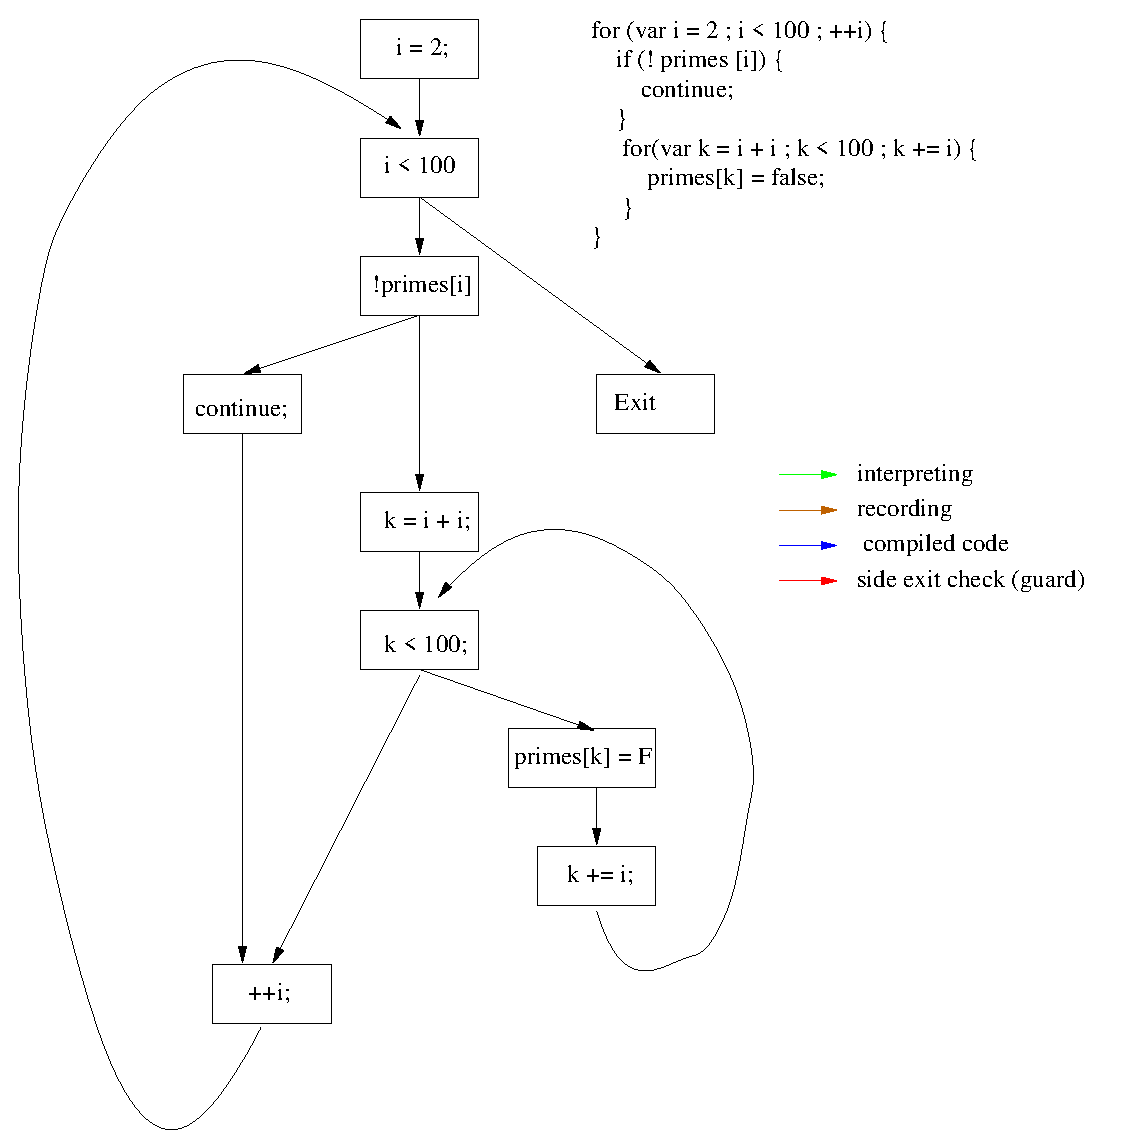
\includegraphics{Figs/1.eps}
  }
  \end{figure}
}
\frame
{
  \begin{figure}[h]
  \centering
  \scalebox{0.45}{
    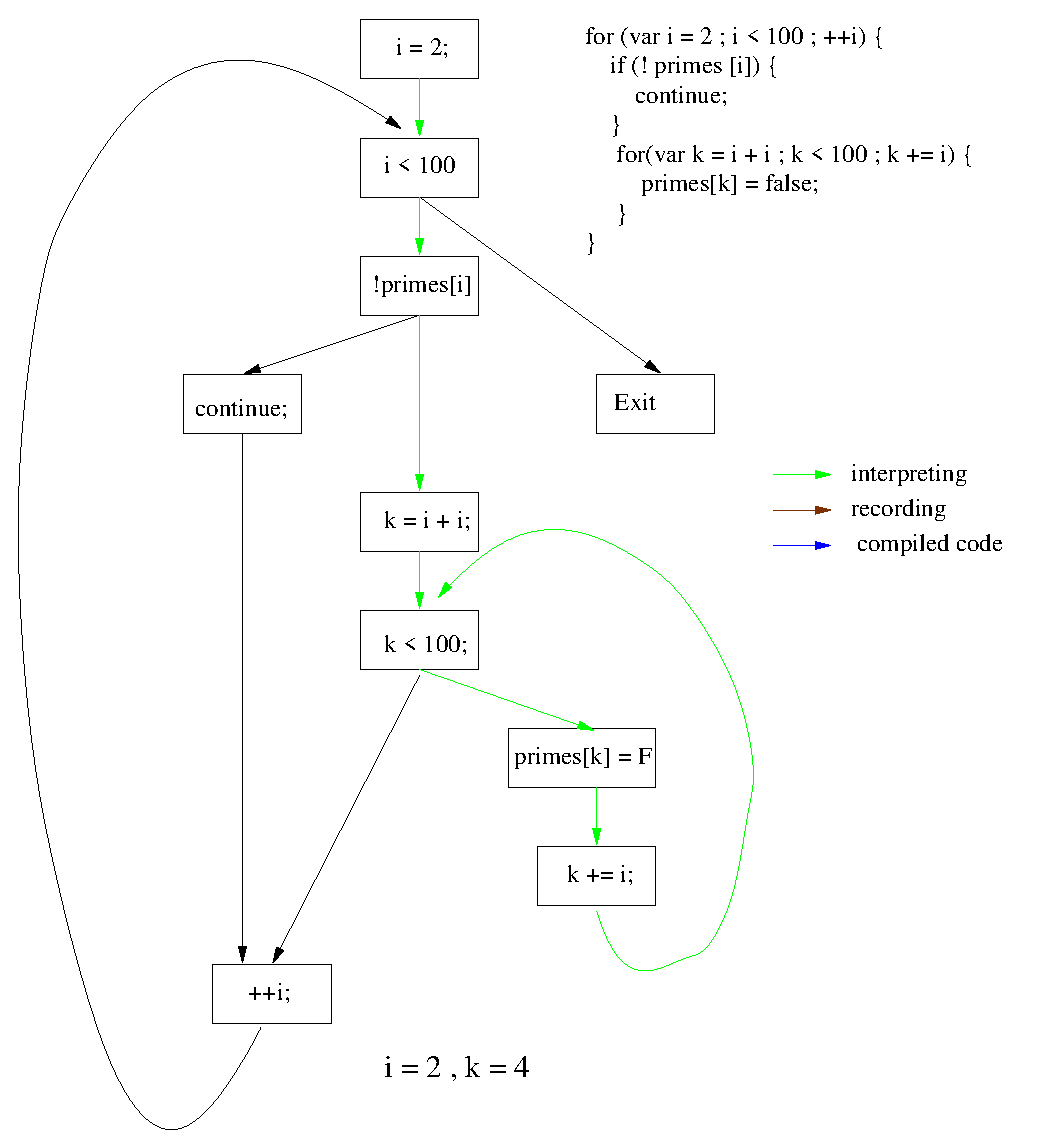
\includegraphics{Figs/1.1.eps}
  }
  \end{figure}
}
\frame
{
  \begin{figure}[h]
  \centering
  \scalebox{0.45}{
    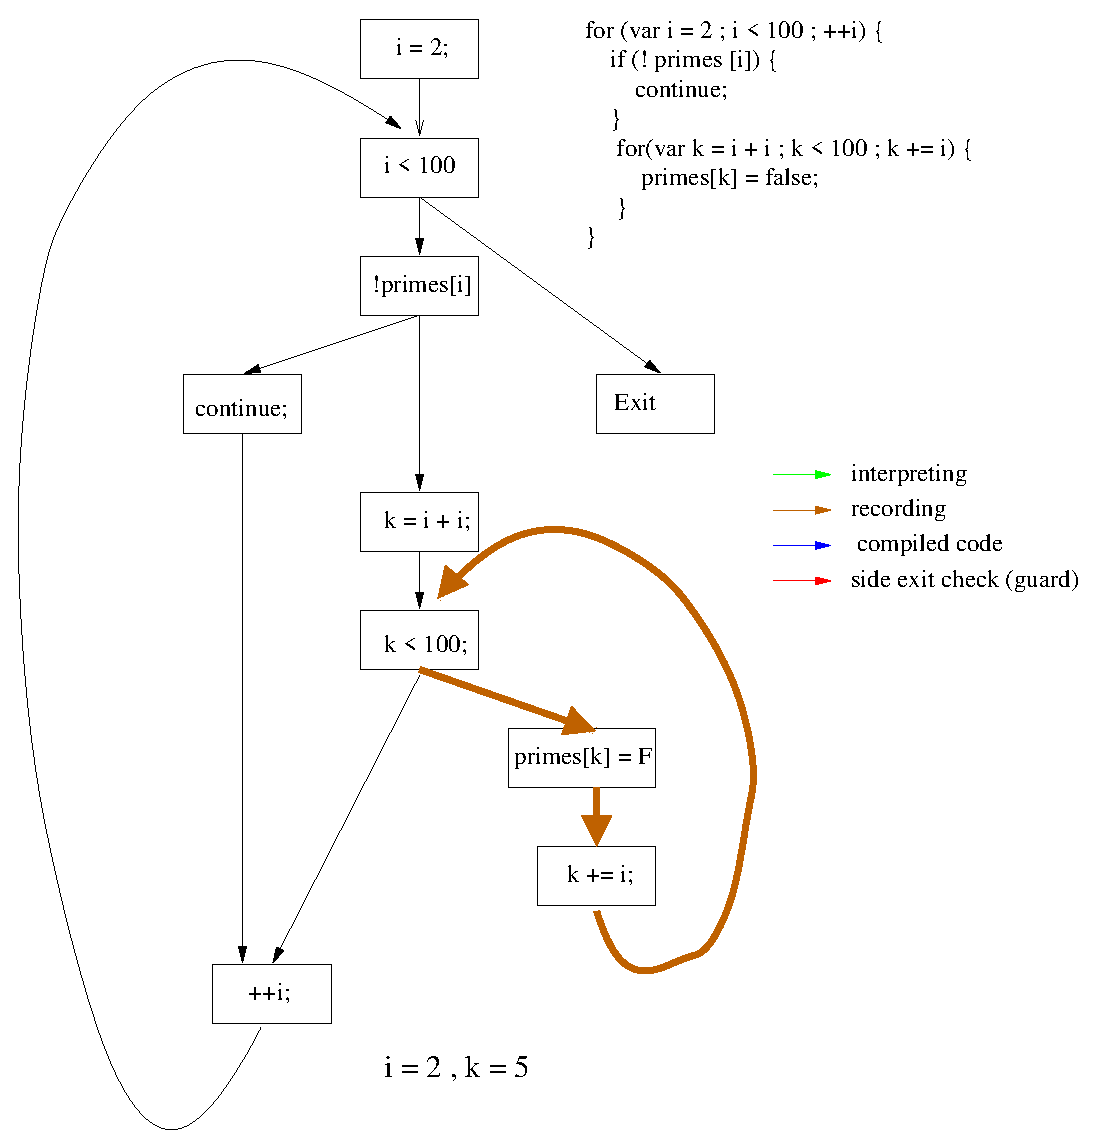
\includegraphics{Figs/1.2.eps}
  }
  \end{figure}
}
\frame
{
  \begin{figure}[h]
  \centering
  \scalebox{0.45}{
    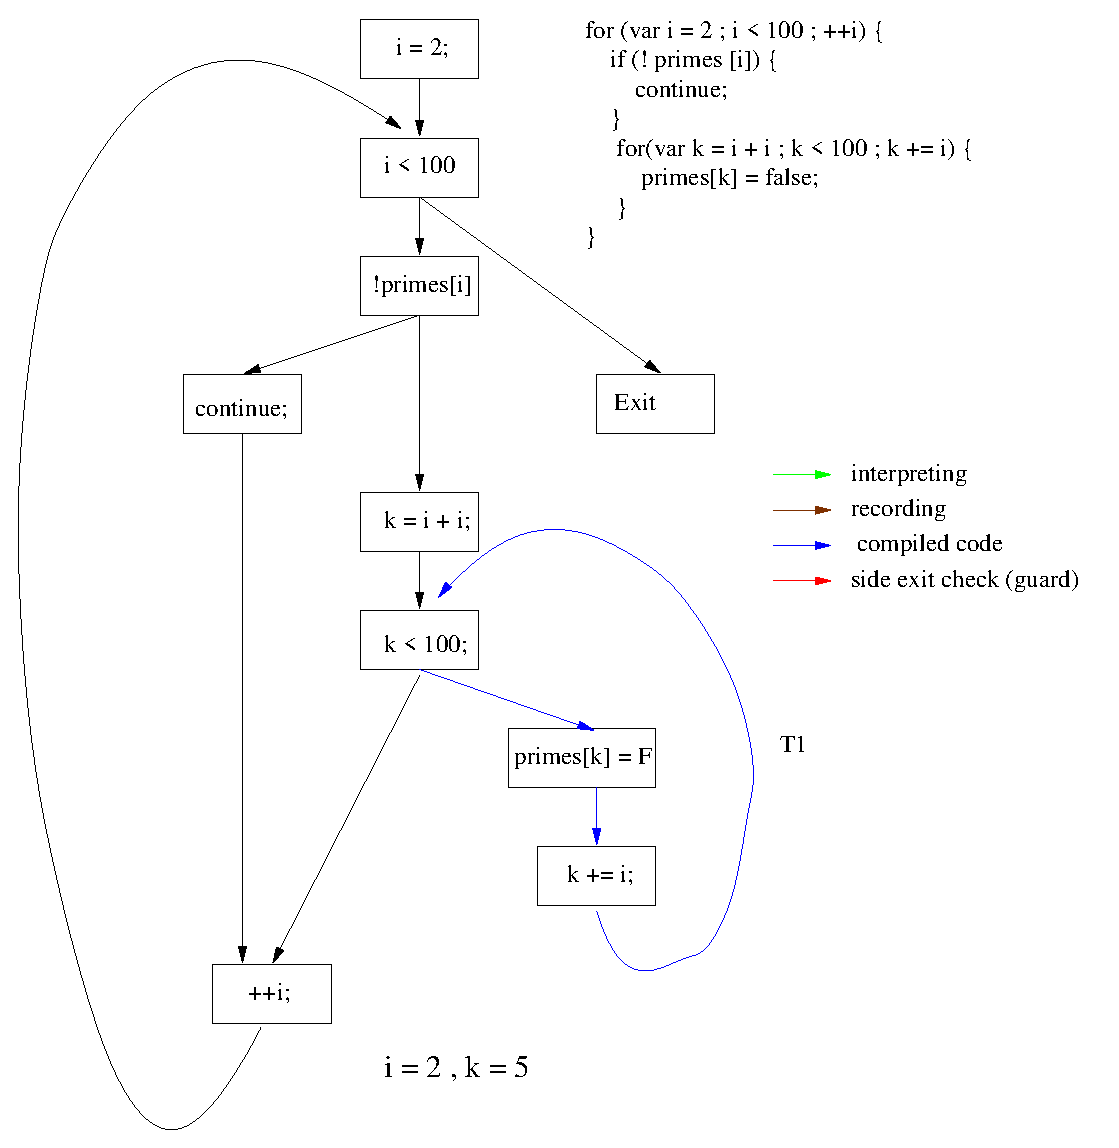
\includegraphics{Figs/1.3.eps}
  }
  \end{figure}
}
\frame
{
  \begin{figure}[h]
  \centering
  \scalebox{0.45}{
    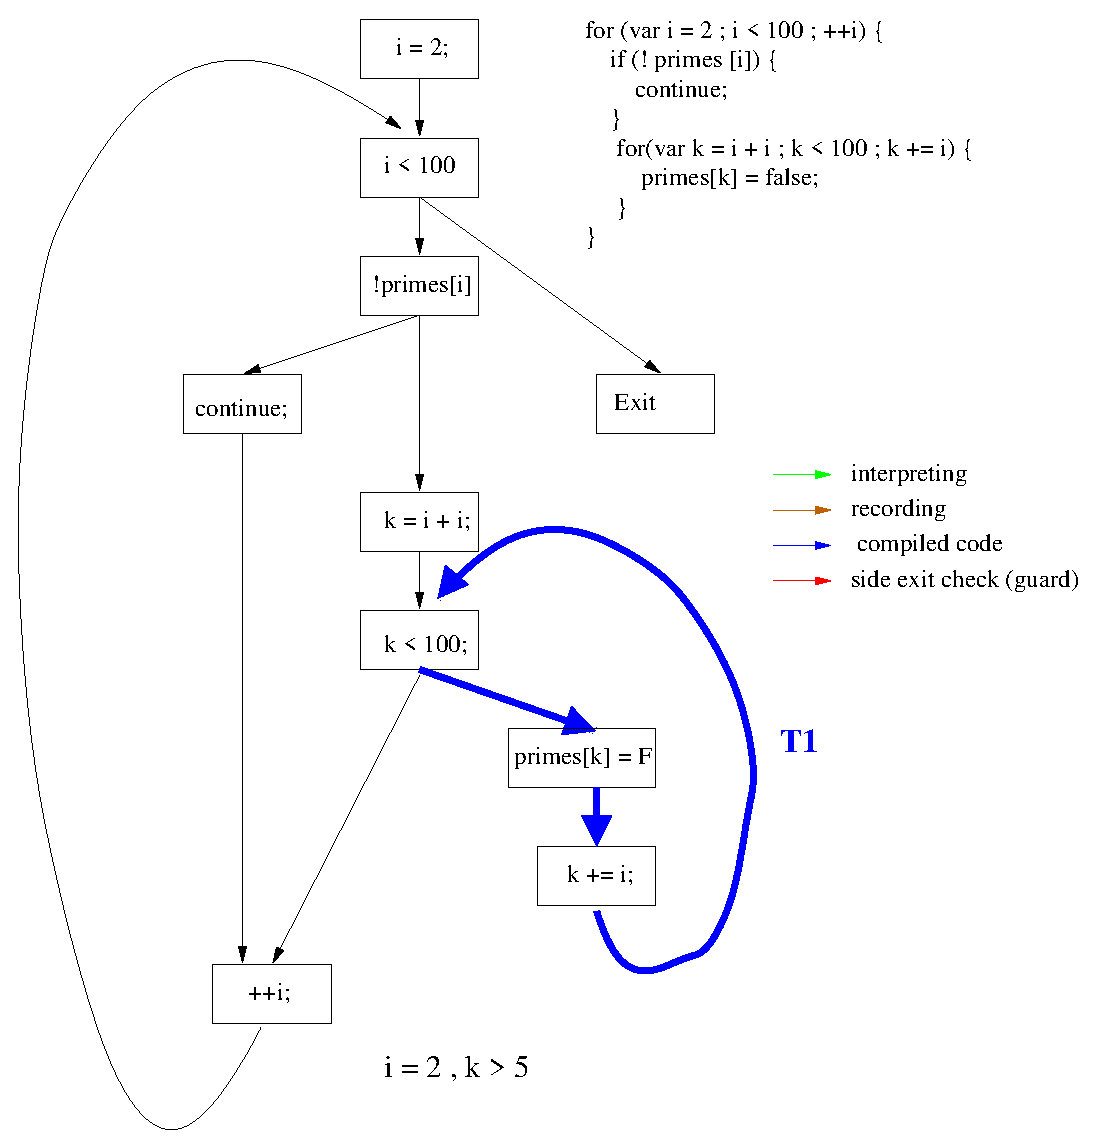
\includegraphics{Figs/1.3.1.eps}
  }
  \end{figure}
}
\frame
{
  \begin{figure}[h]
  \centering
  \scalebox{0.45}{
    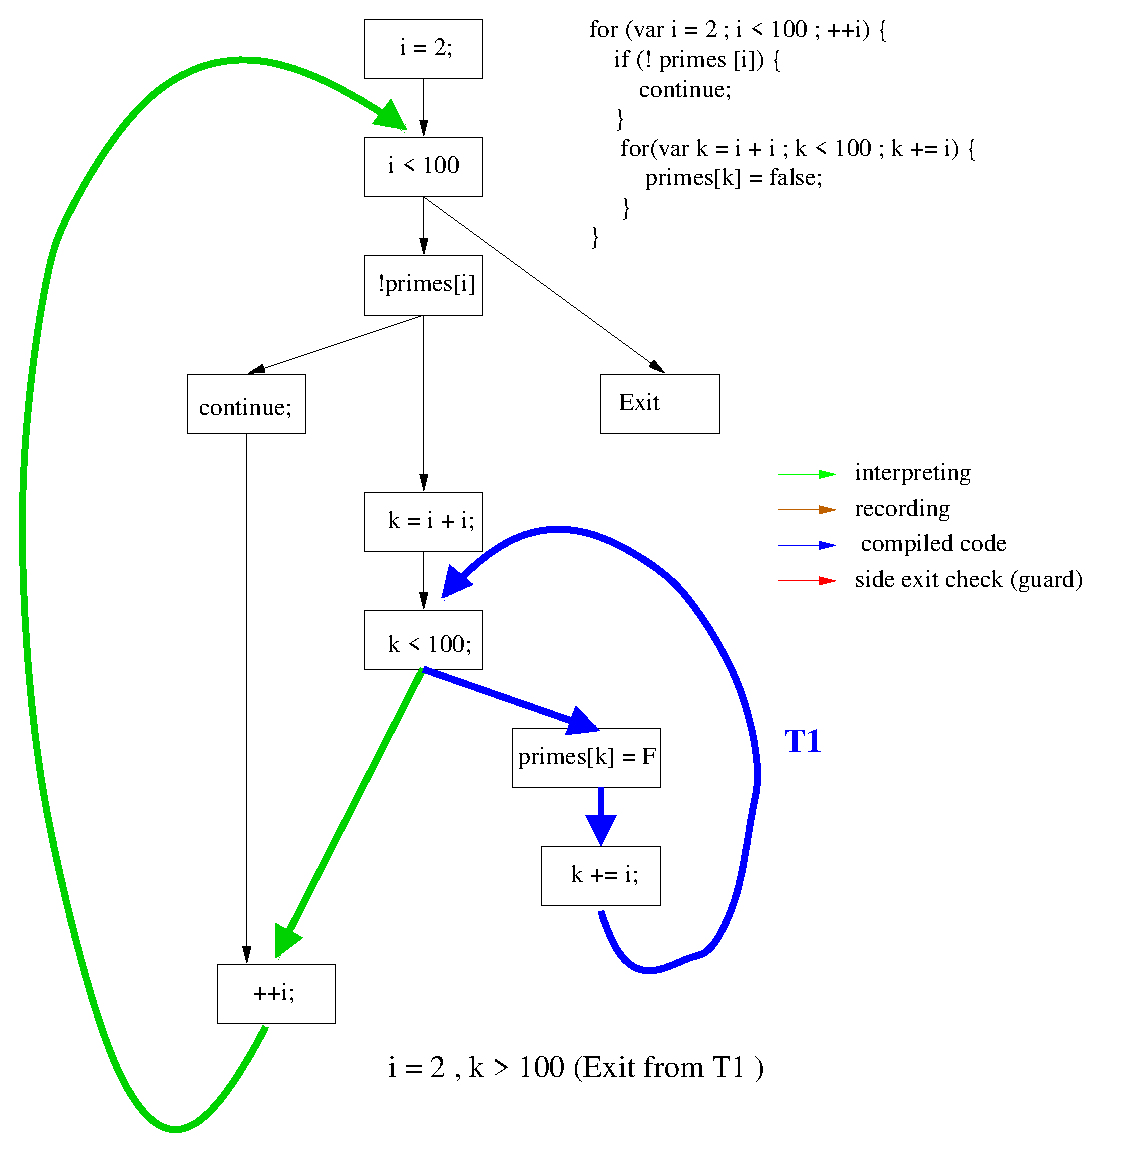
\includegraphics{Figs/1.3.2.eps}
  }
  \end{figure}
}
\frame
{
  \begin{figure}[h]
  \centering
  \scalebox{0.45}{
    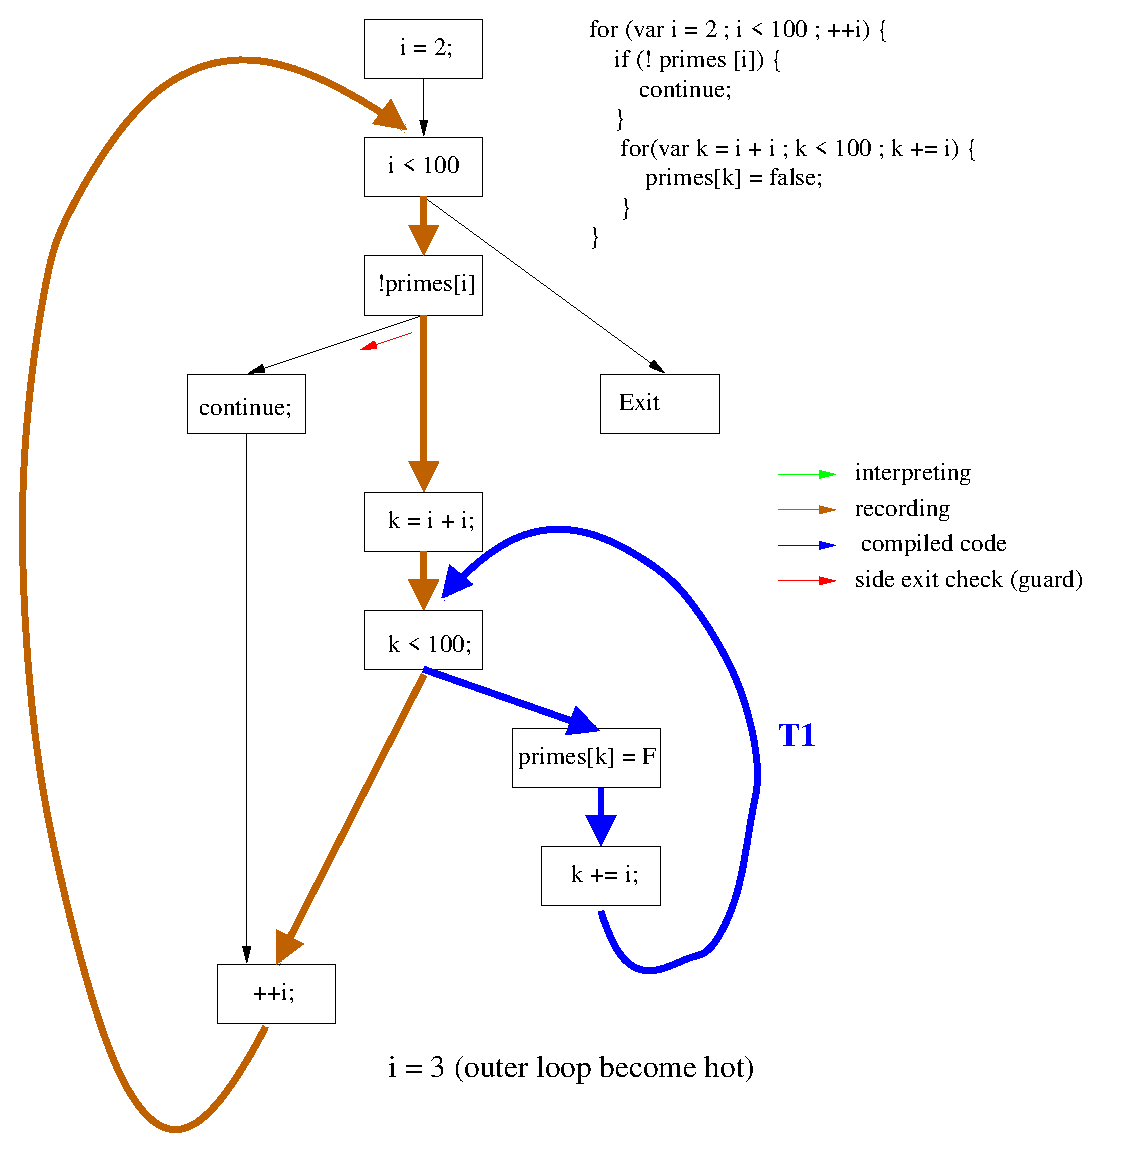
\includegraphics{Figs/1.4.eps}
  }
  \end{figure}
}
\frame
{
  \begin{figure}[h]
  \centering
  \scalebox{0.45}{
    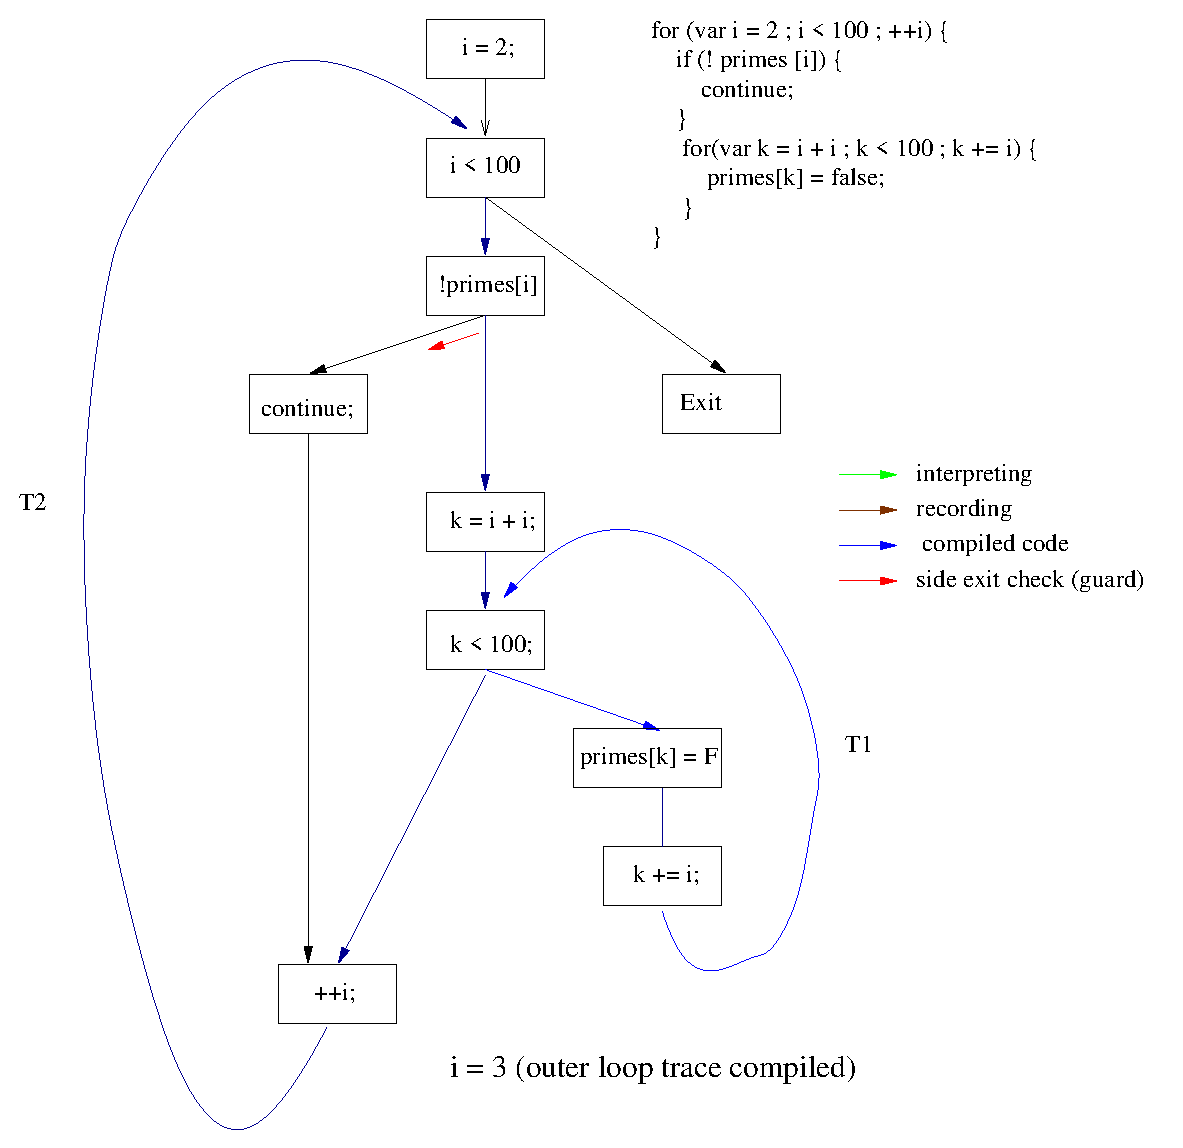
\includegraphics{Figs/1.5.eps}
  }
  \end{figure}
}
\frame
{
  \begin{figure}[h]
  \centering
  \scalebox{0.45}{
    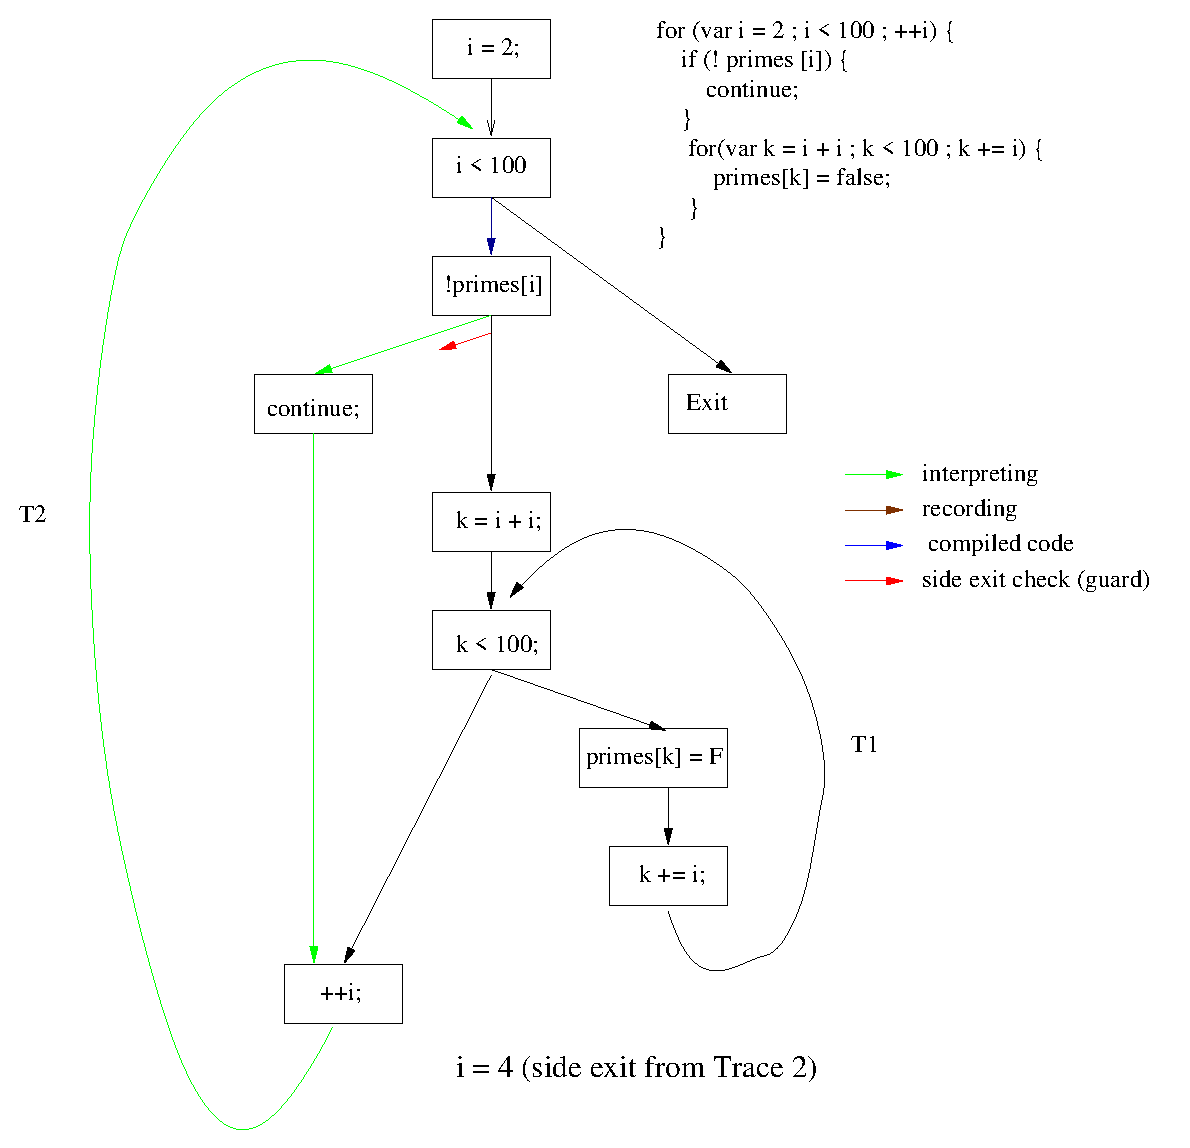
\includegraphics{Figs/1.6.eps}
  }
  \end{figure}
}
\frame
{
  \begin{figure}[h]
  \centering
  \scalebox{0.45}{
    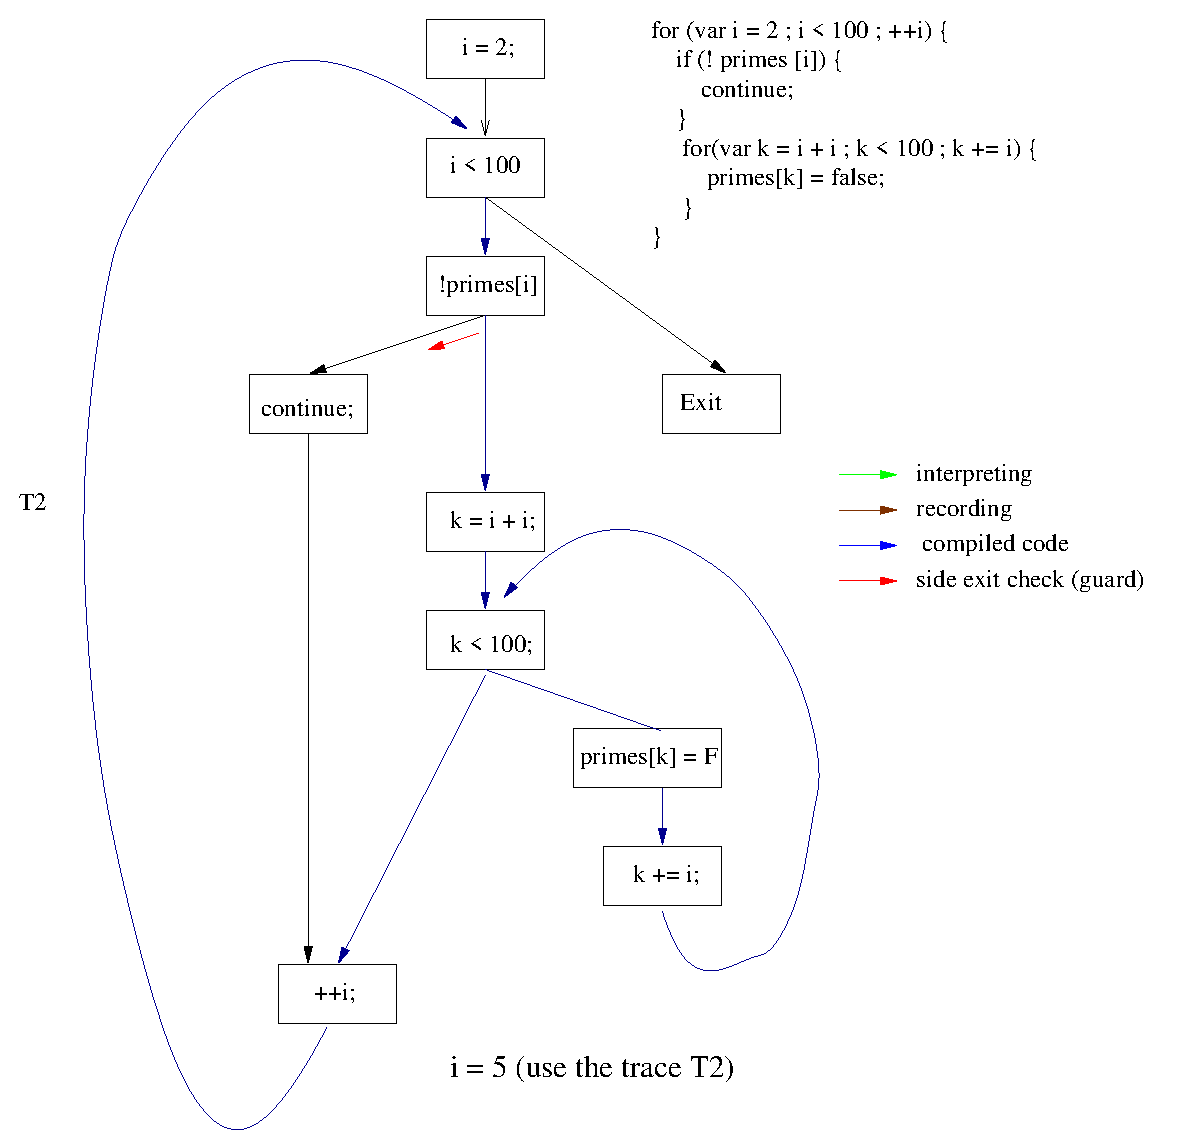
\includegraphics{Figs/1.7.eps}
  }
  \end{figure}
}
\frame
{
  \begin{figure}[h]
  \centering
  \scalebox{0.45}{
    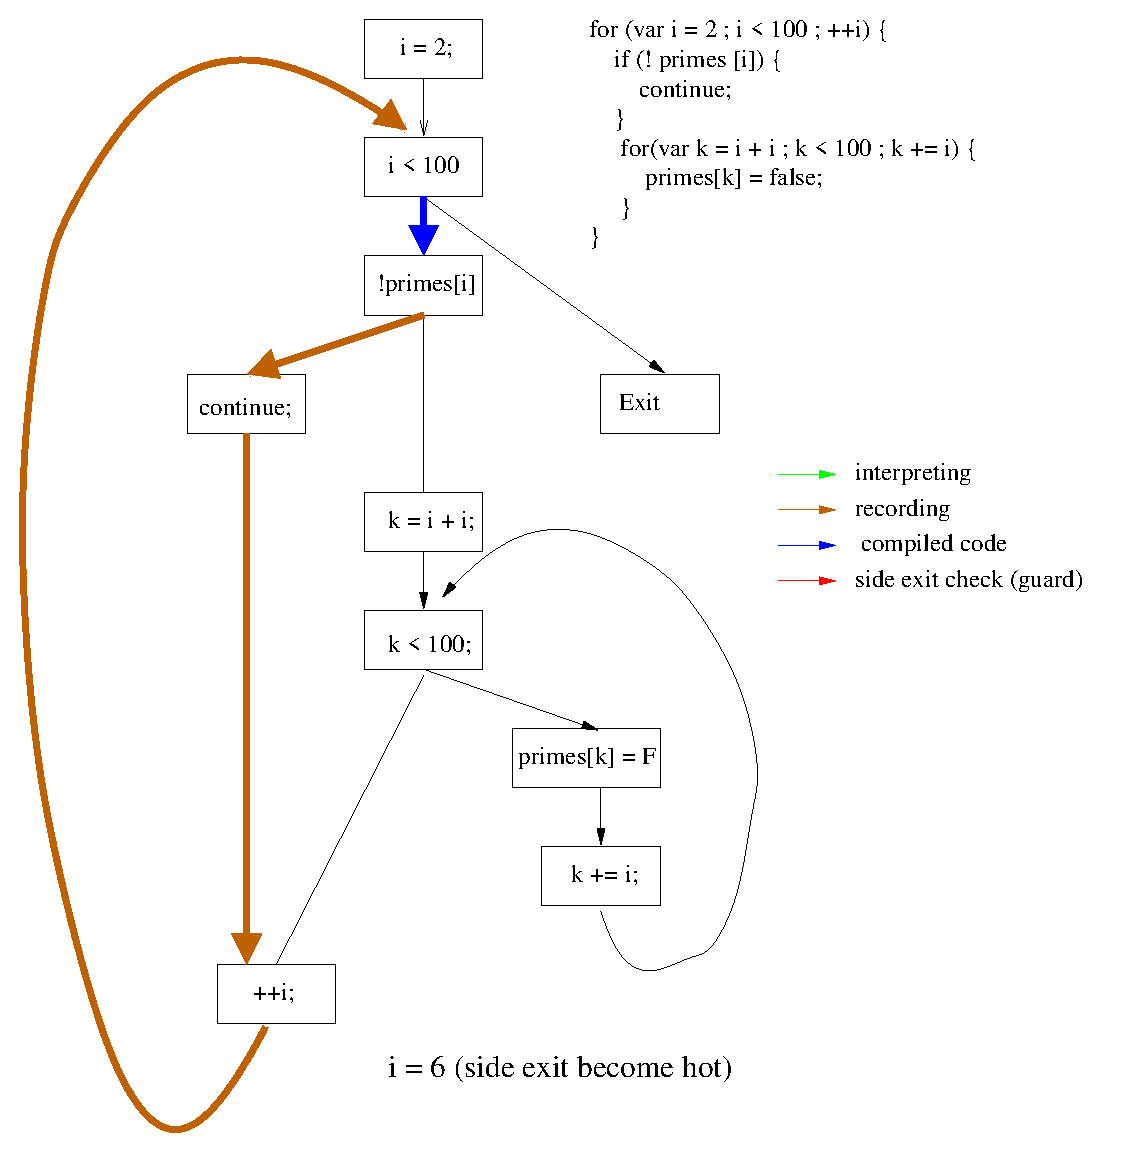
\includegraphics{Figs/1.8.eps}
  }
  \end{figure}
}
\frame
{
  \begin{figure}[h]
  \centering
  \scalebox{0.45}{
    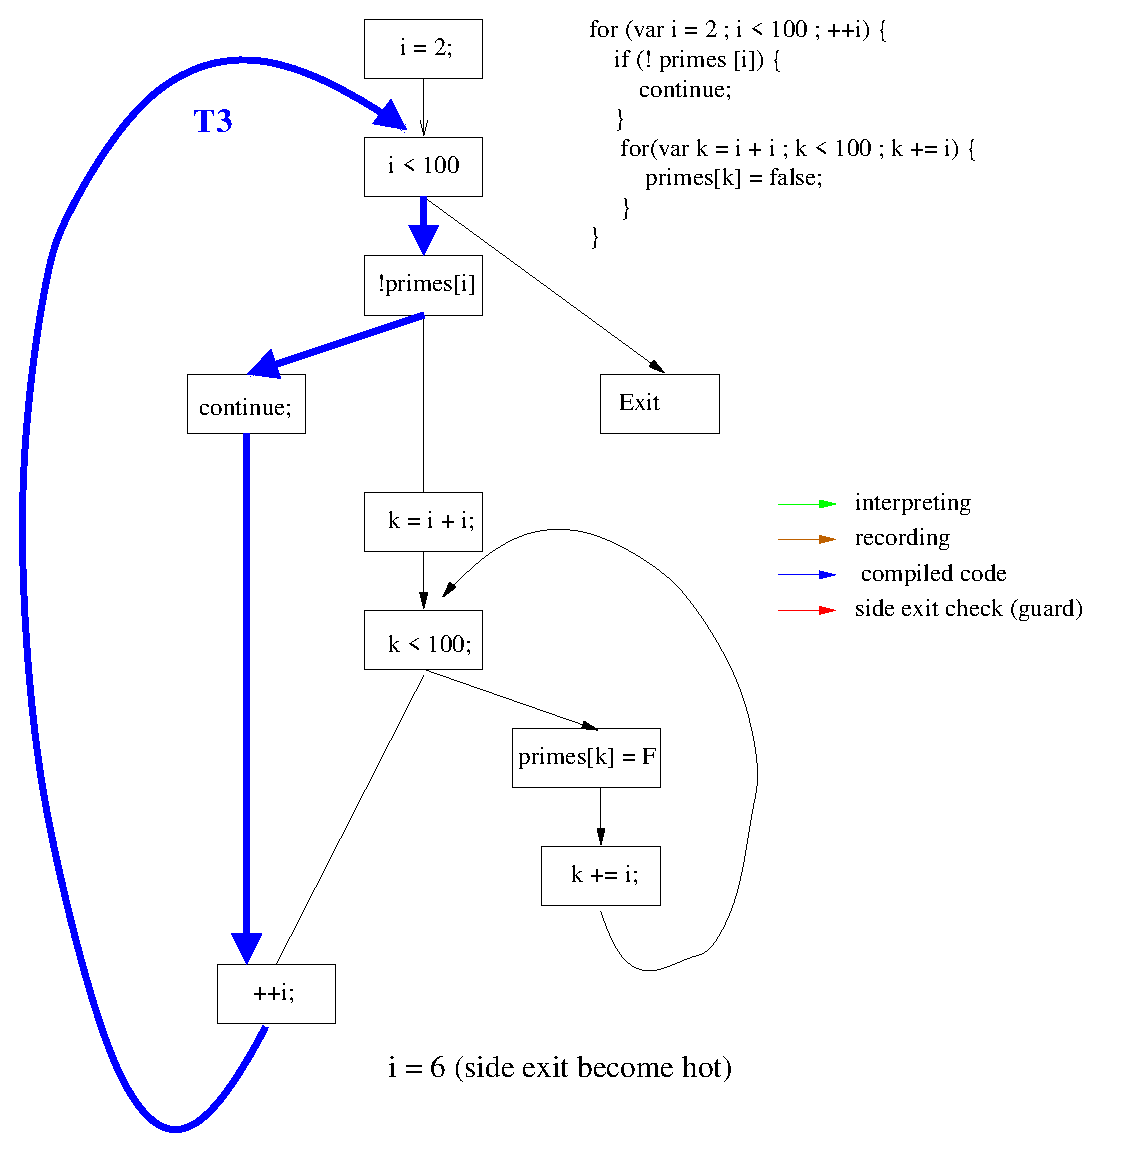
\includegraphics{Figs/1.9.eps}
  }
  \end{figure}
}

\section{Trace Tree Formation}
\subsection{Type Stable Trace}
\frame
{
  \frametitle{\subsecname}
  \begin{figure}[h]
  \centering
  \scalebox{0.45}{
    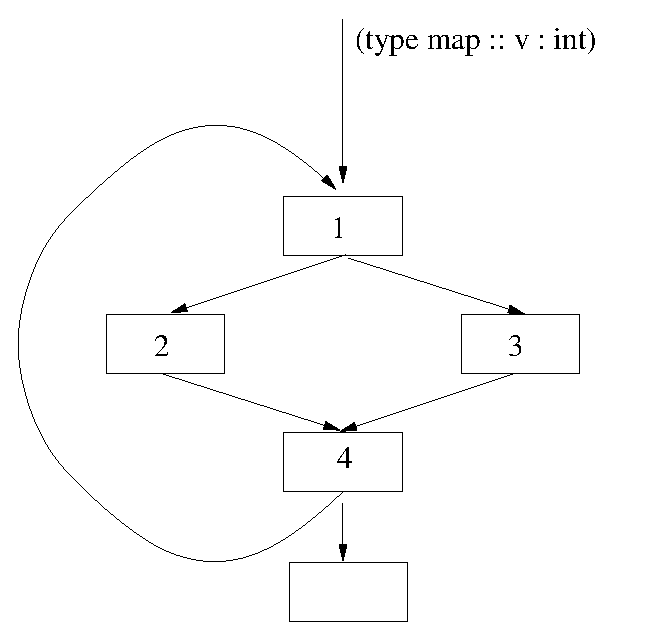
\includegraphics{Figs/4.1.eps}
  }
  \end{figure}
}
\frame
{
  \frametitle{\subsecname}
  \begin{figure}[h]
  \centering
  \scalebox{0.45}{
    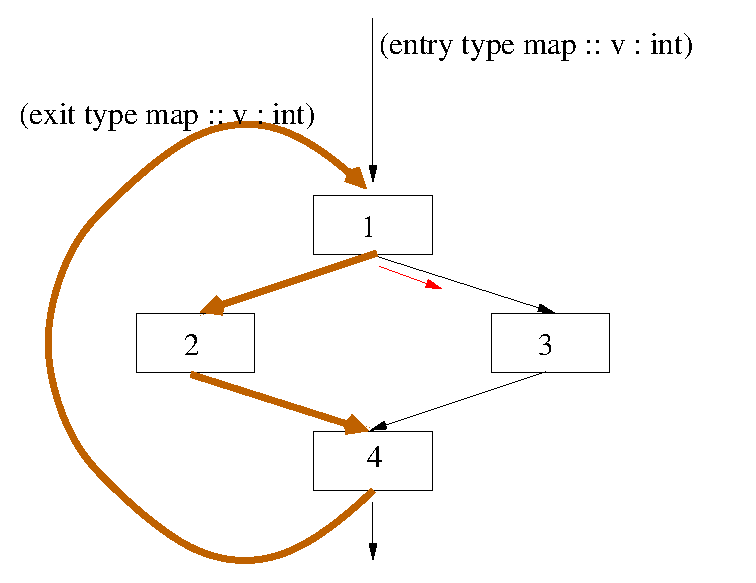
\includegraphics{Figs/4.2.eps}
  }
  \end{figure}
}
\frame
{
  \frametitle{\subsecname}
  \begin{figure}[h]
  \centering
  \scalebox{0.45}{
    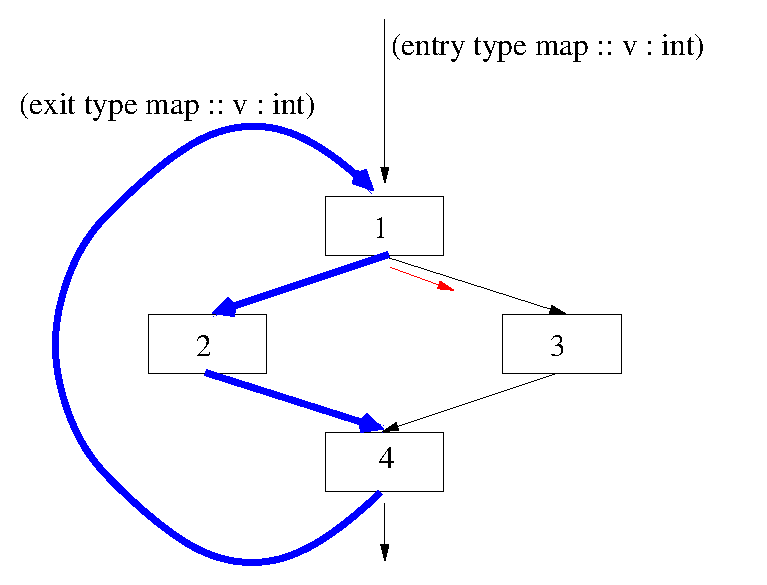
\includegraphics{Figs/4.3.eps}
  }
  \end{figure}
}
\subsection{Trace Tree Extension}
\frame
{
  \frametitle{\subsecname}
  \begin{figure}[h]
  \centering
  \scalebox{0.45}{
    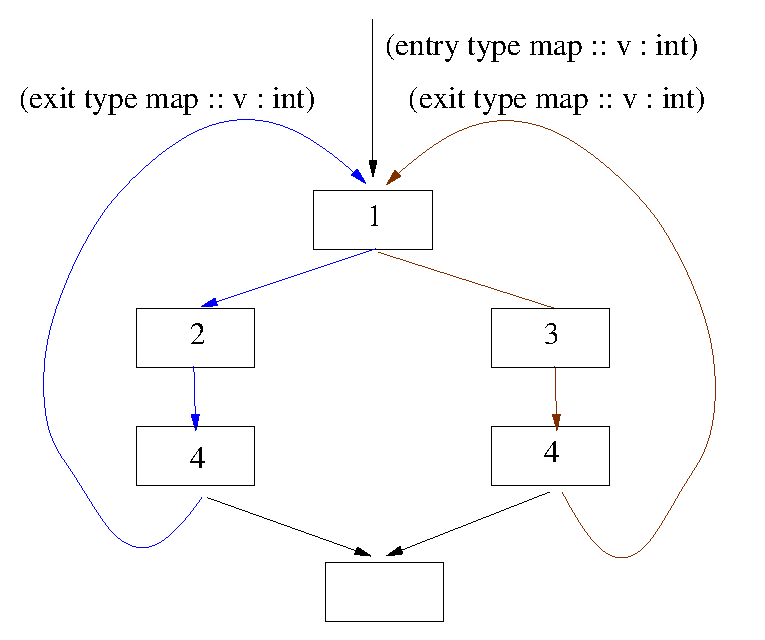
\includegraphics{Figs/4.4.eps}
  }
  \end{figure}
Note: Current Implepentation extends only if 
        \begin{itemize}
          \item side exit is for control flow branch
          \item does not leave the loop
        \end{itemize}
}
\subsection{Type Unstable Trace Handling}
\frame
{
  \frametitle{\subsecname}
  \begin{figure}[h]
  \centering
  \scalebox{0.45}{
    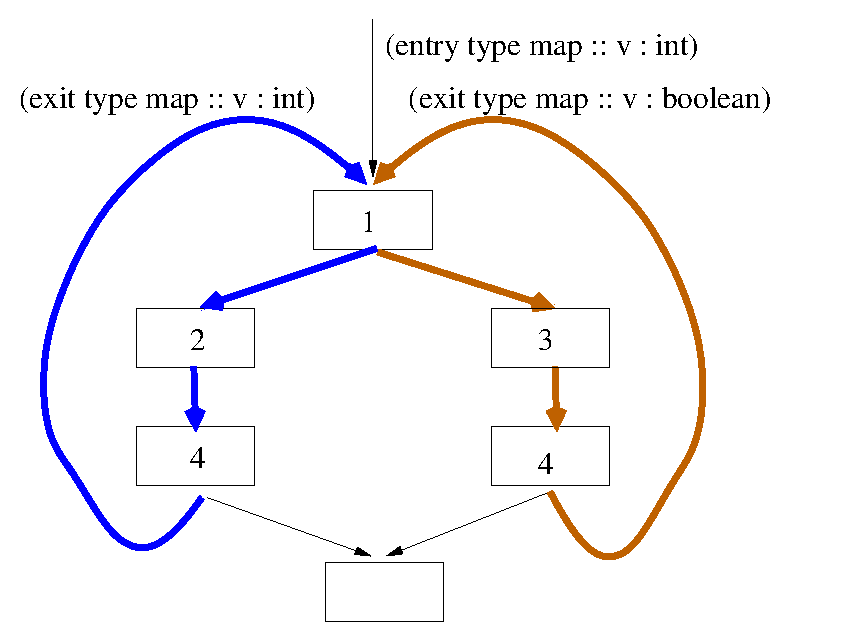
\includegraphics{Figs/4.5.eps}
  }
  \end{figure}
}
\frame
{
  \frametitle{\subsecname}
  \begin{figure}[h]
  \centering
  \scalebox{0.45}{
    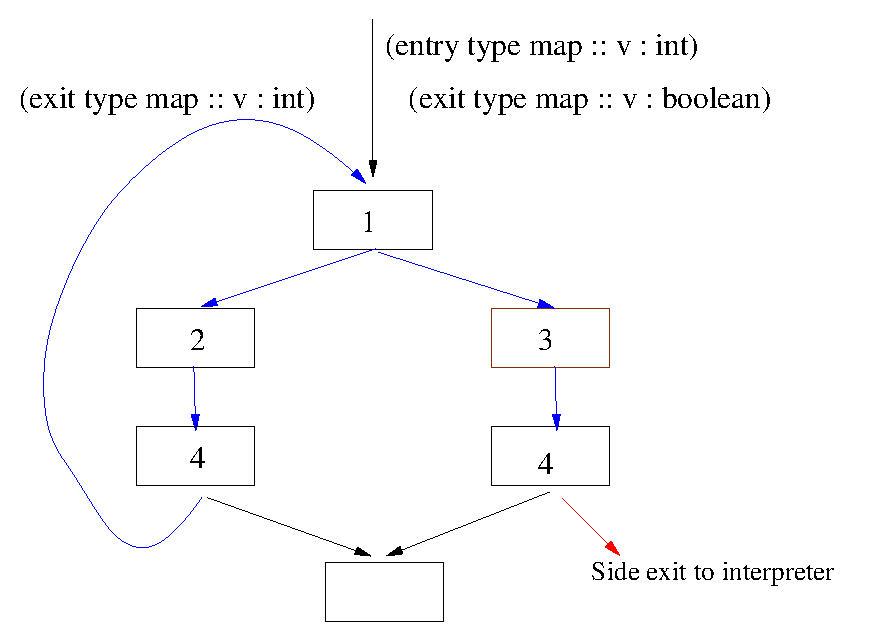
\includegraphics{Figs/4.5.1.eps}
  }
  \end{figure}
}
\frame
{
  \frametitle{\subsecname}
  \begin{figure}[h]
  \centering
  \scalebox{0.45}{
    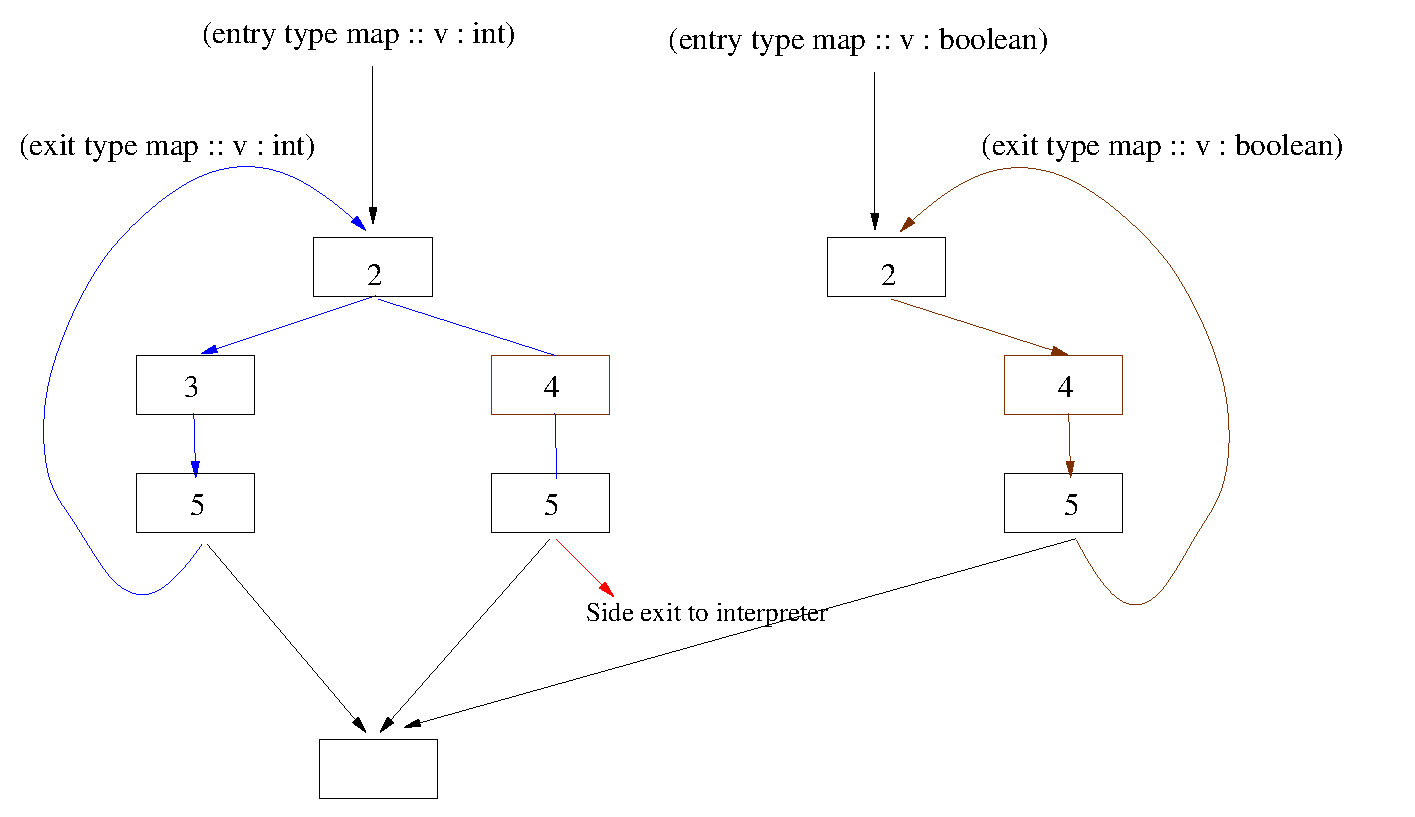
\includegraphics{Figs/4.6.eps}
  }
  \end{figure}
}
\frame
{
  \frametitle{\subsecname}
  \begin{figure}[h]
  \centering
  \scalebox{0.45}{
    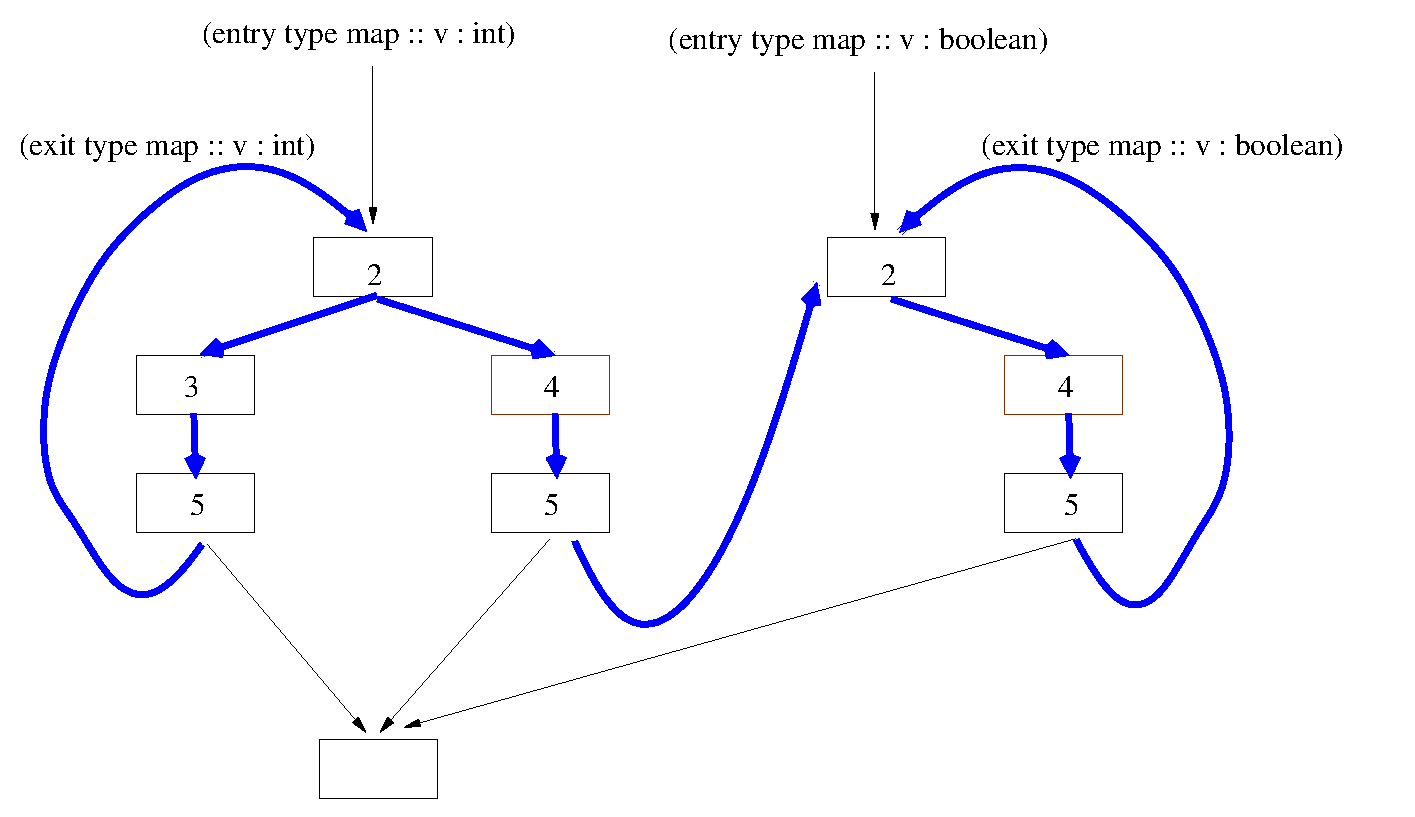
\includegraphics{Figs/4.7.eps}
  }
  \end{figure}
}
\subsection{Blacklisting}
\frame
{
  \frametitle{\subsecname}
  \begin{itemize}
   \item What if a hot loop contain traces that always fail recording ? 
   \uncover<2> { \item Solution : Blacklist with backoff on recording }
   \end{itemize}
}
\cmt{recording overhead is huge.}

\section{Nested Trace Tree Formation}
\frame
{
  \frametitle{\secname}
  \begin{figure}[h]
  \centering
  \scalebox{0.45}{
    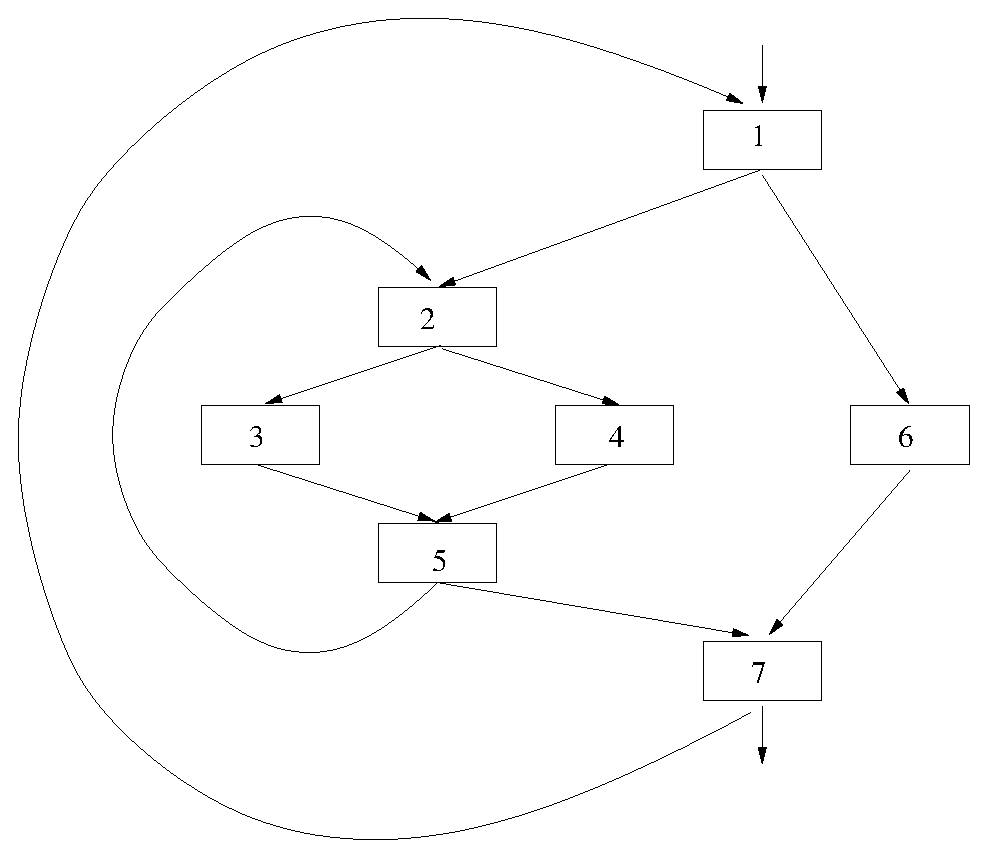
\includegraphics{Figs/2.1.eps}
  }
  \end{figure}

  
}
\frame
{
  \frametitle{\secname}
  \begin{figure}[h]
  \centering
  \scalebox{0.45}{
    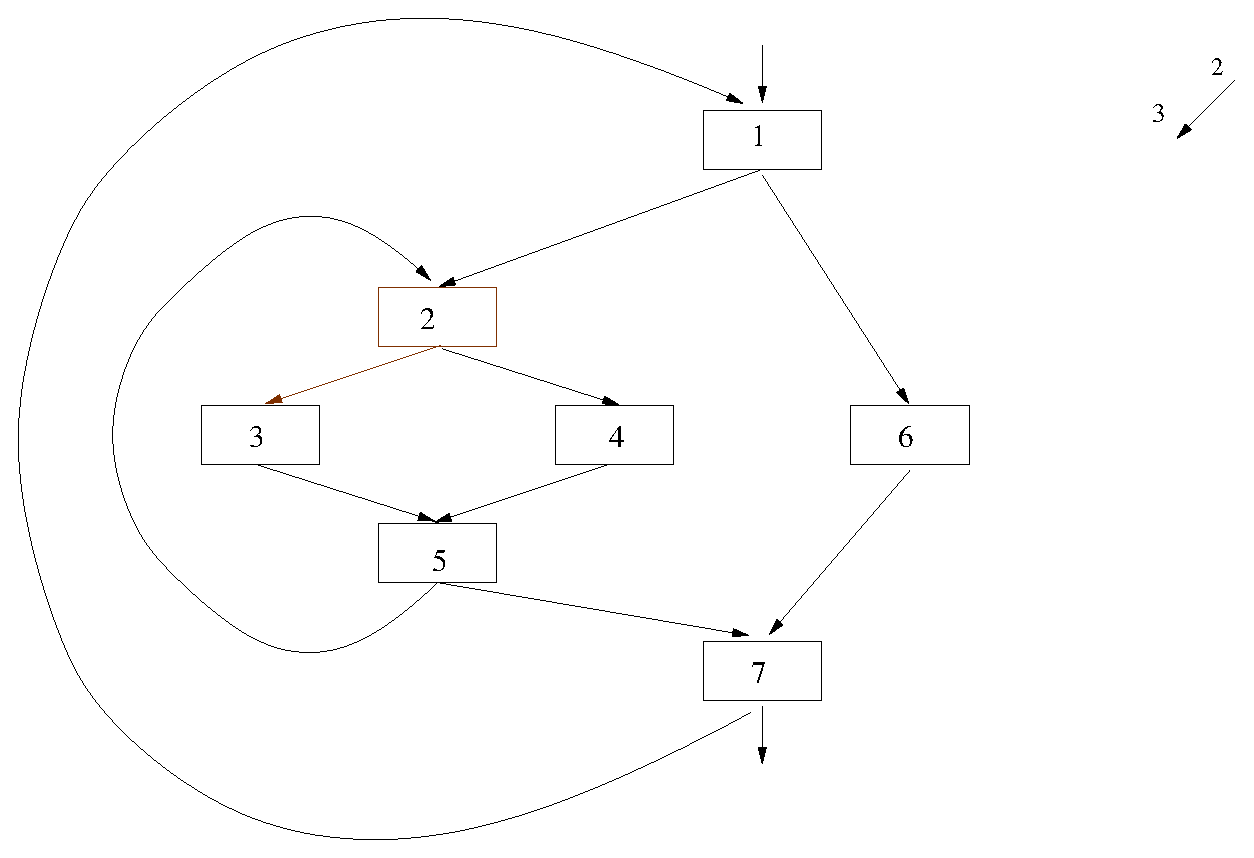
\includegraphics{Figs/2.2.eps}
  }
  \end{figure}
}
\frame
{
  \frametitle{\secname}
  \begin{figure}[h]
  \centering
  \scalebox{0.45}{
    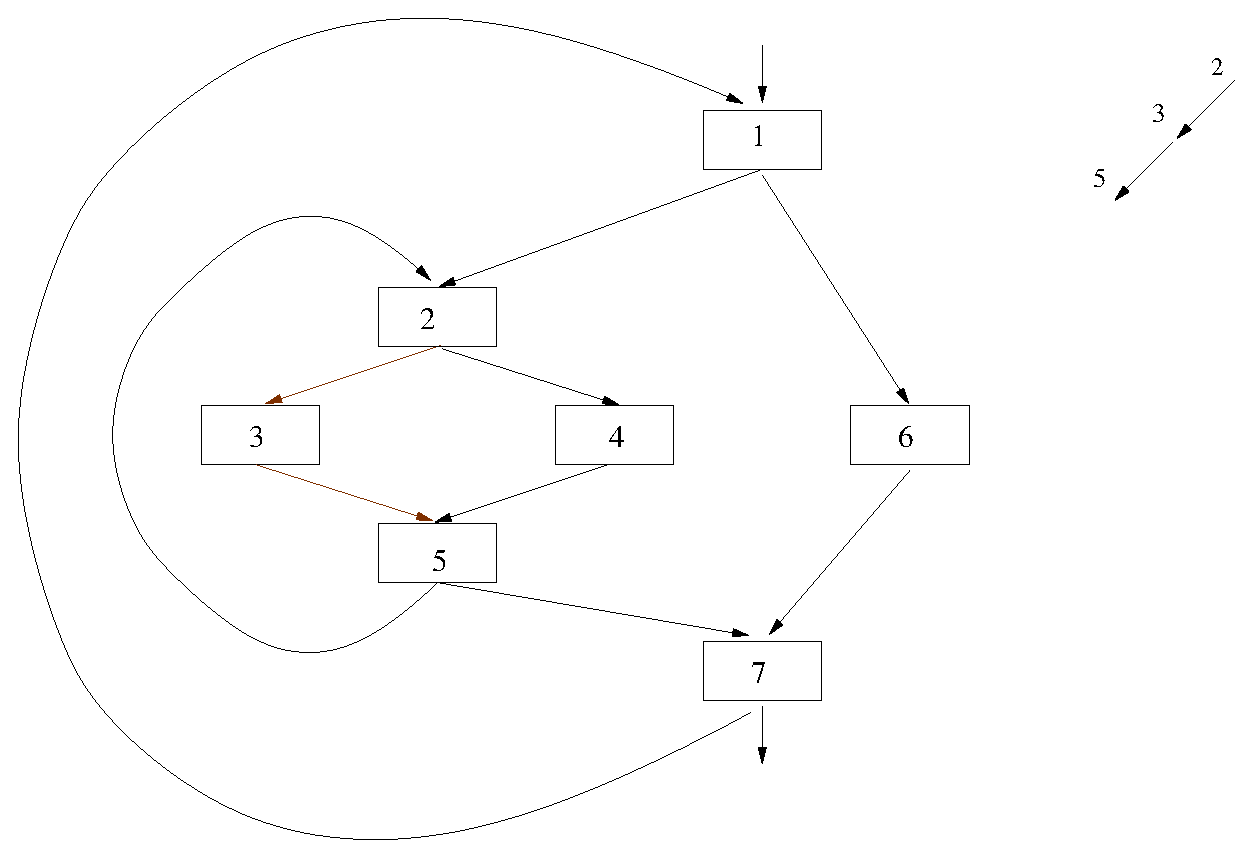
\includegraphics{Figs/2.3.eps}
  }
  \end{figure}
}
\frame
{
  \frametitle{\secname}
  \begin{figure}[h]
  \centering
  \scalebox{0.45}{
    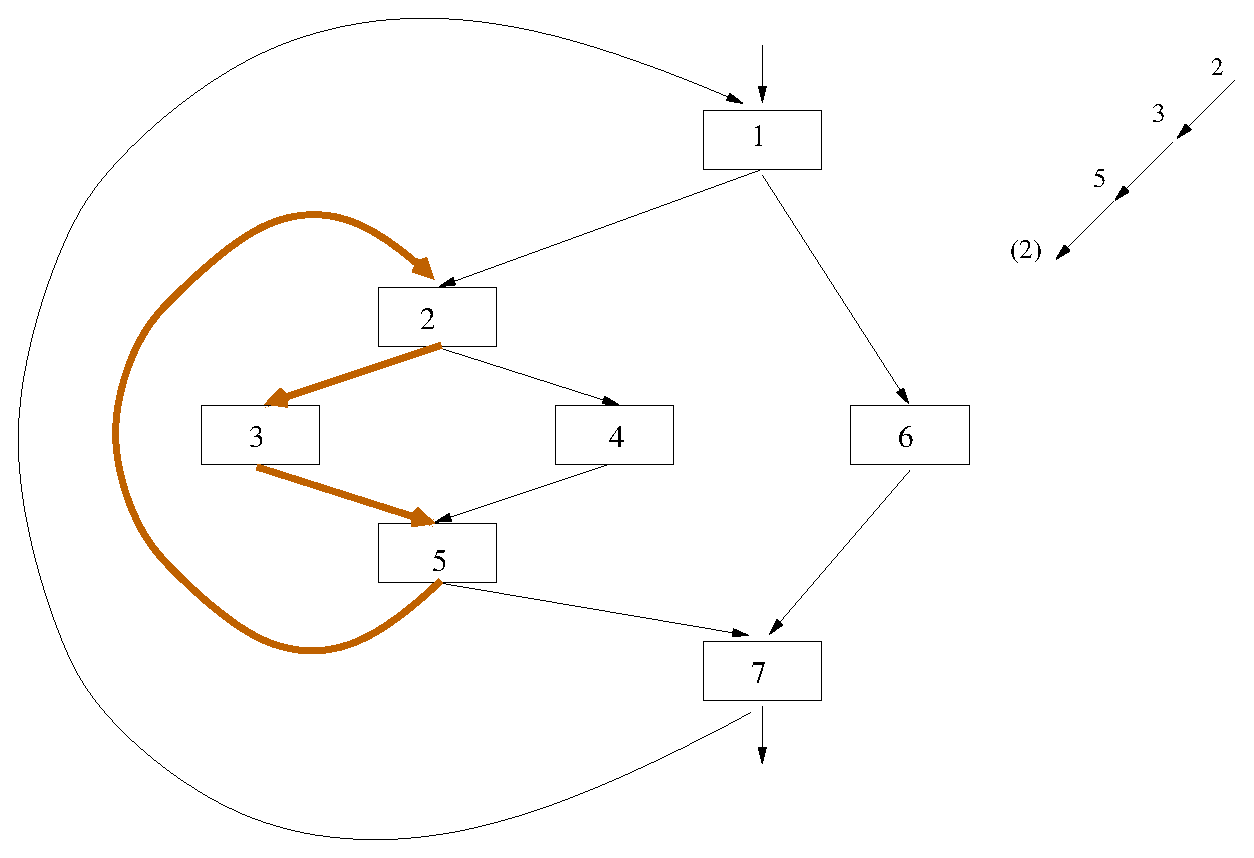
\includegraphics{Figs/2.4.eps}
  }
  \end{figure}
}
\frame
{
  \frametitle{\secname}
  \begin{figure}[h]
  \centering
  \scalebox{0.45}{
    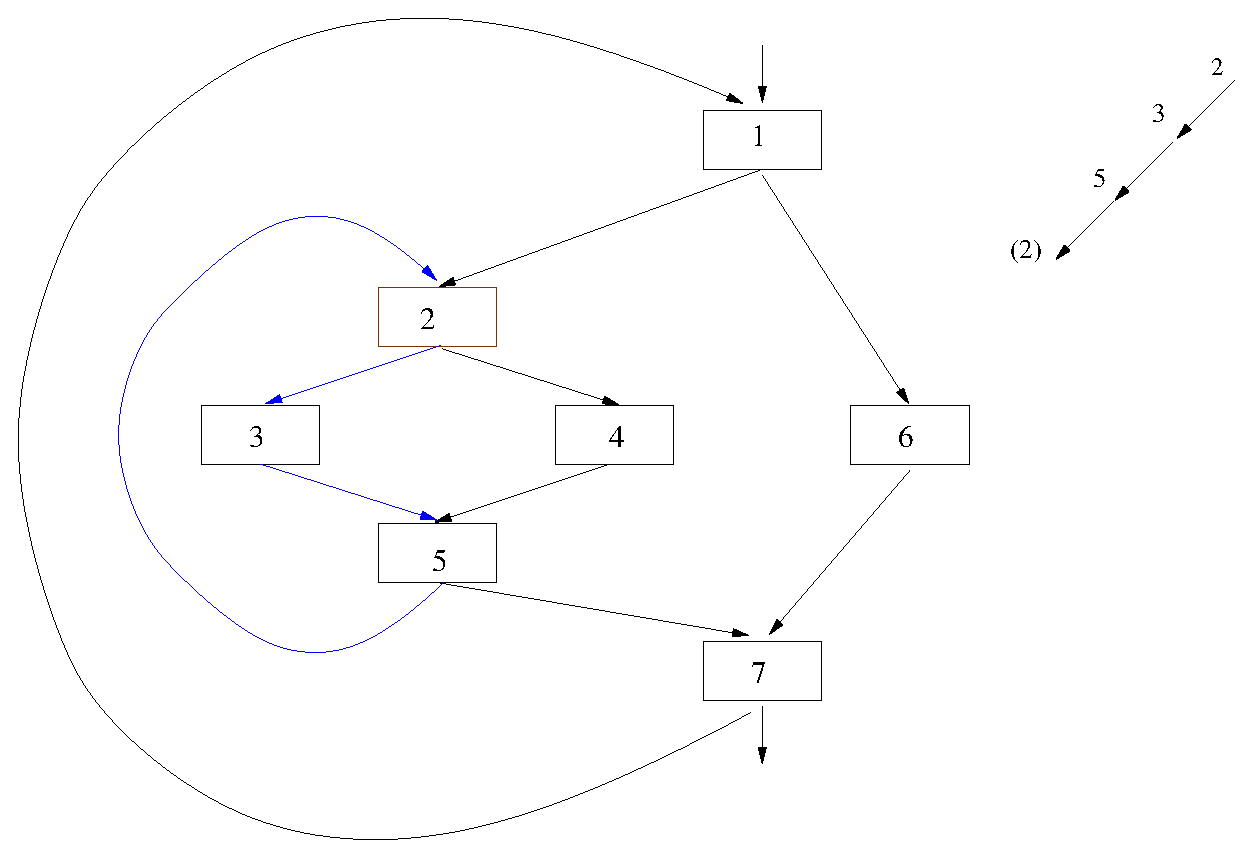
\includegraphics{Figs/2.4.1.eps}
  }
  \end{figure}
}
\subsection{Continue tracing for outer loop}
\frame
{
  \frametitle{\subsecname}
  \begin{figure}[h]
  \centering
  \scalebox{0.45}{
    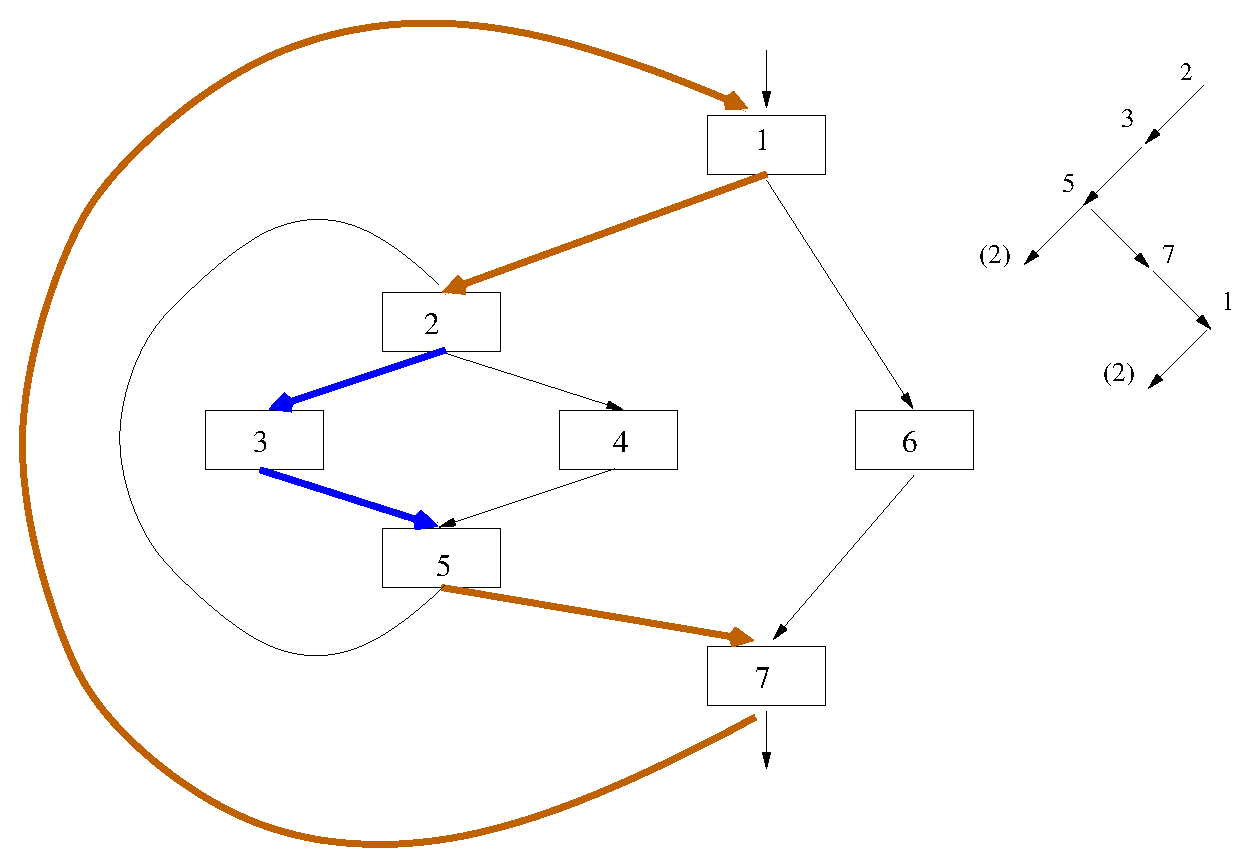
\includegraphics{Figs/2.5.eps}
  }
  \end{figure}
}
\frame
{
  \begin{figure}[h]
  \centering
  \scalebox{0.45}{
    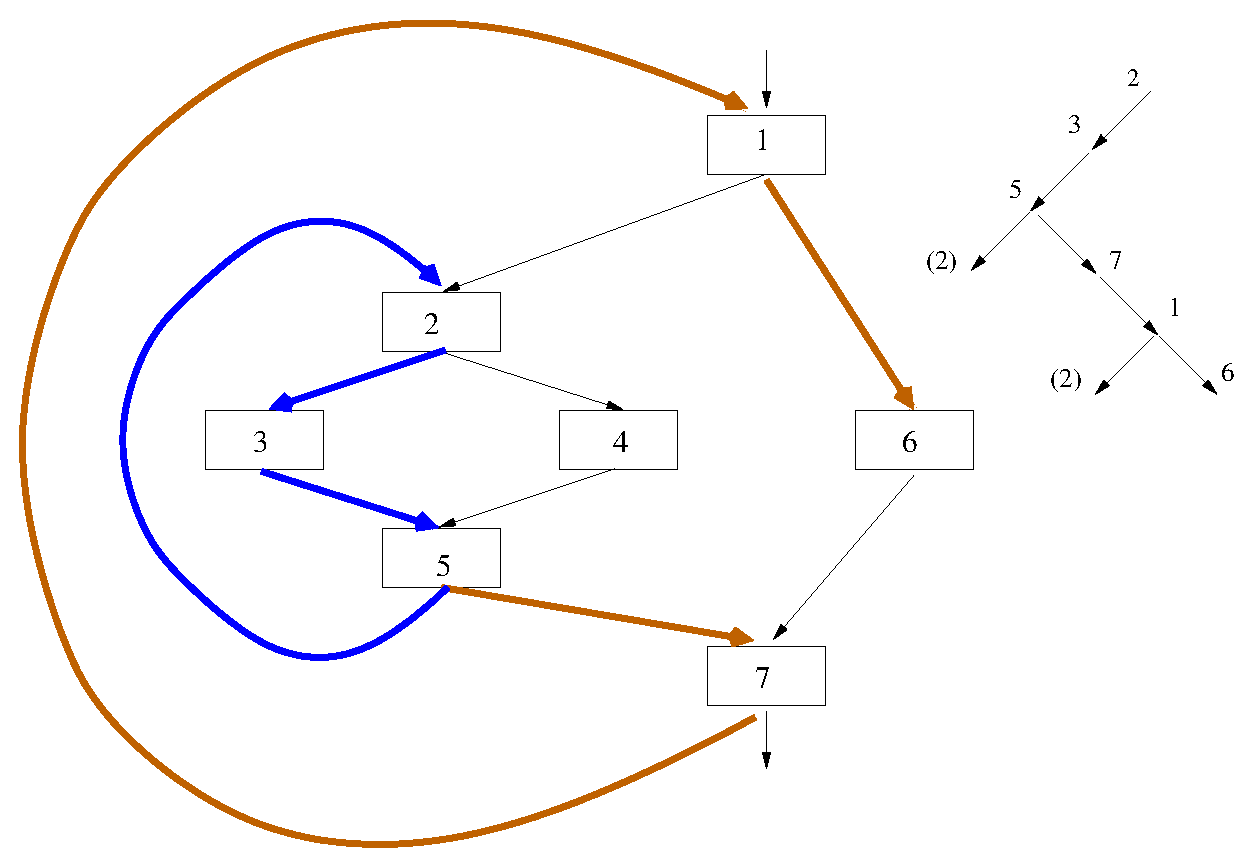
\includegraphics{Figs/2.7.eps}
  }
  \end{figure}
}
\frame
{
  \frametitle{\subsecname}
  \begin{figure}[h]
  \centering
  \scalebox{0.45}{
    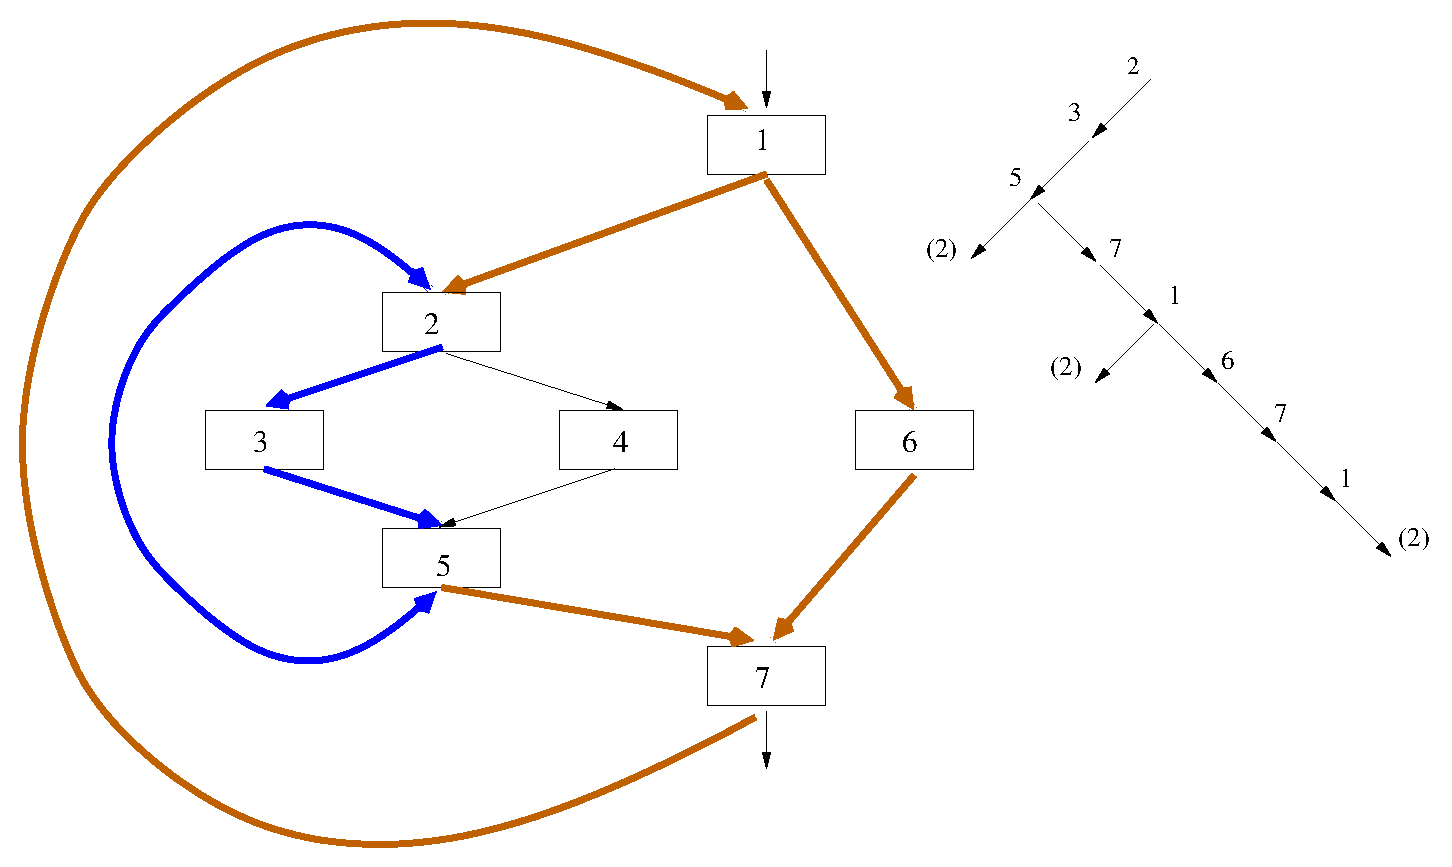
\includegraphics{Figs/2.8.eps}
  }
  \end{figure}
}
\frame
{
  \frametitle{\subsecname}
  \begin{figure}[h]
  \centering
  \scalebox{0.45}{
    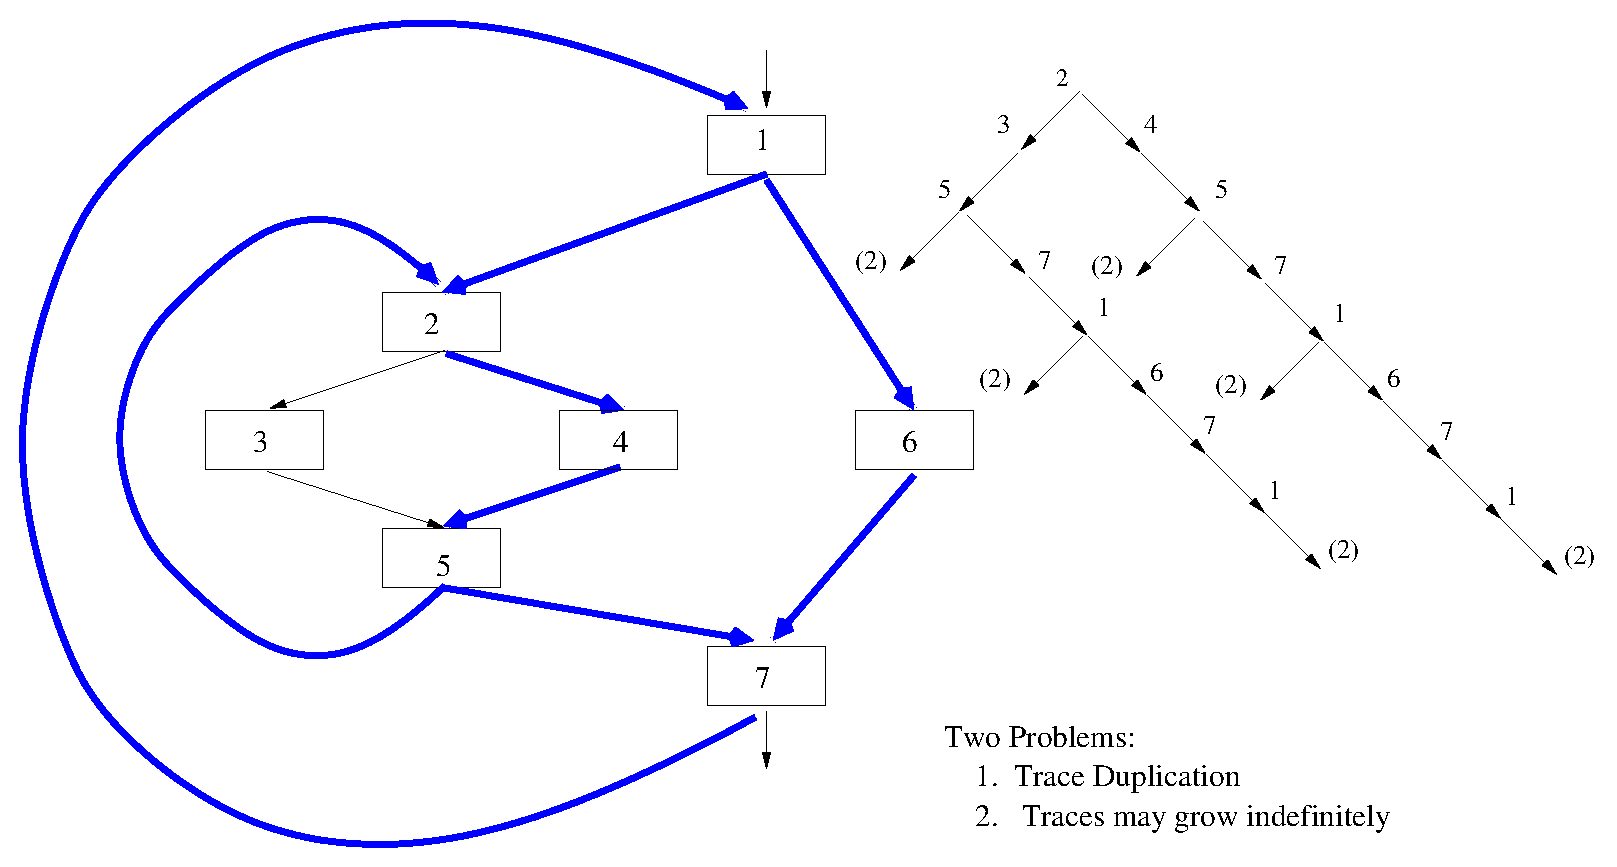
\includegraphics{Figs/2.9.eps}
  }
  \end{figure}

}

\subsection{Separate traces}
\frame
{
  \frametitle{\subsecname}
  \begin{figure}[h]
  \centering
  \scalebox{0.45}{
    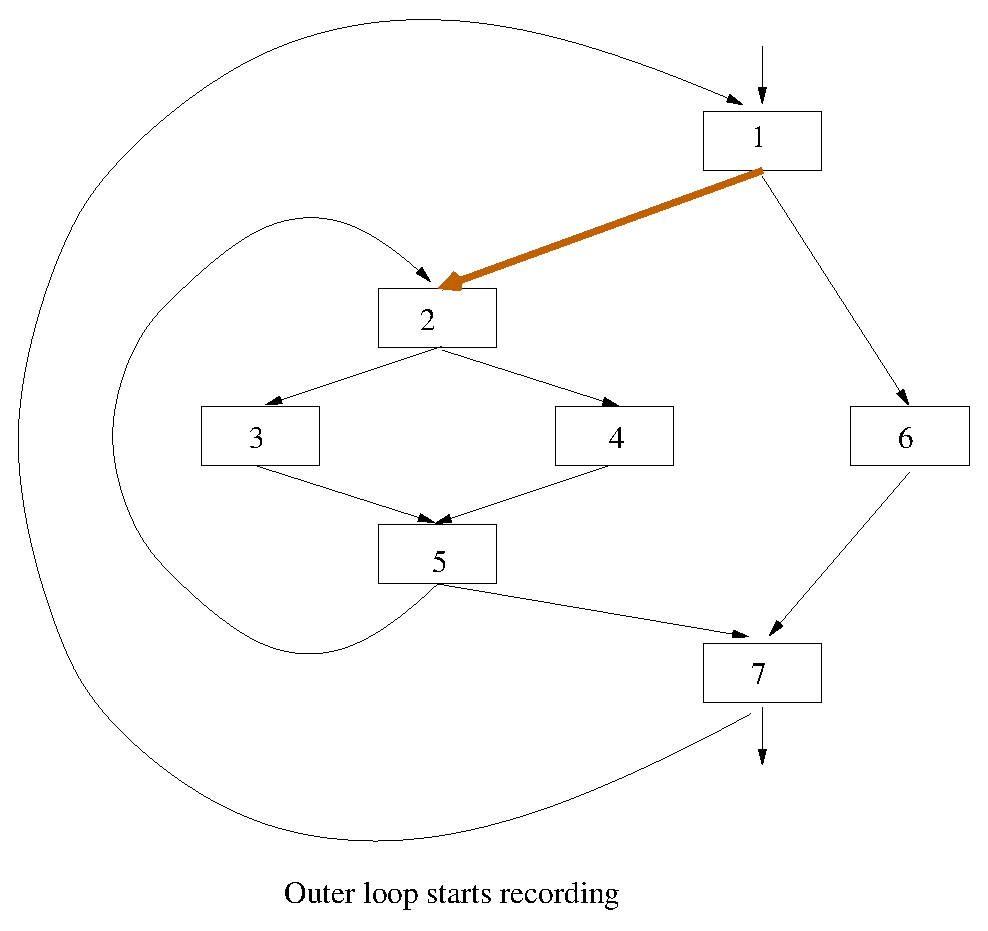
\includegraphics{Figs/3.1.eps}
  }
  \end{figure}
}
\frame
{
  \frametitle{\subsecname}
  \begin{figure}[h]
  \centering
  \scalebox{0.45}{
    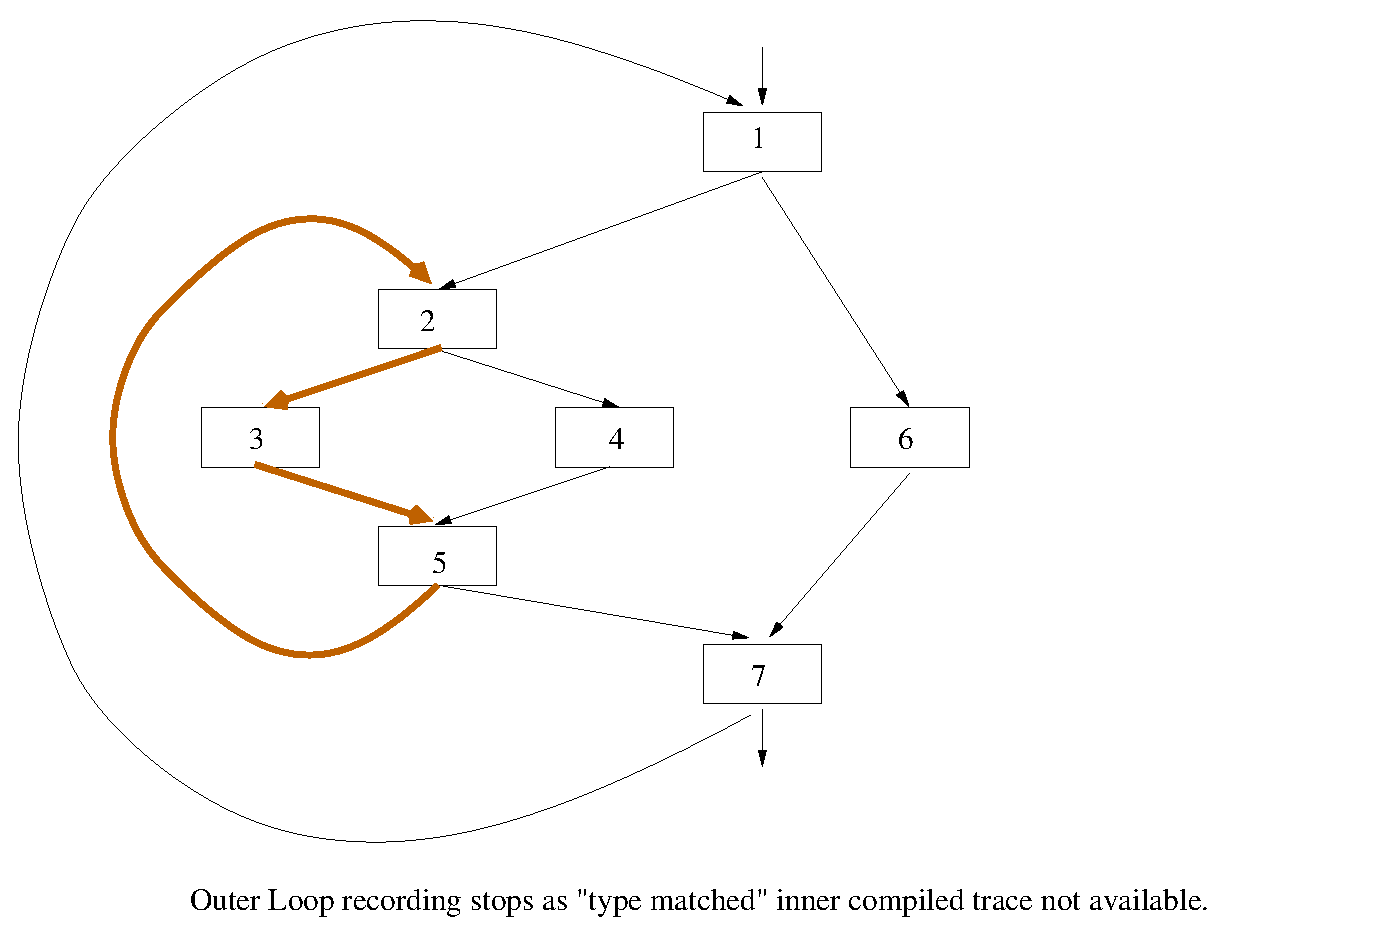
\includegraphics{Figs/3.2.eps}
  }
  \end{figure}
}
\frame
{
  \frametitle{\subsecname}
  \begin{figure}[h]
  \centering
  \scalebox{0.45}{
    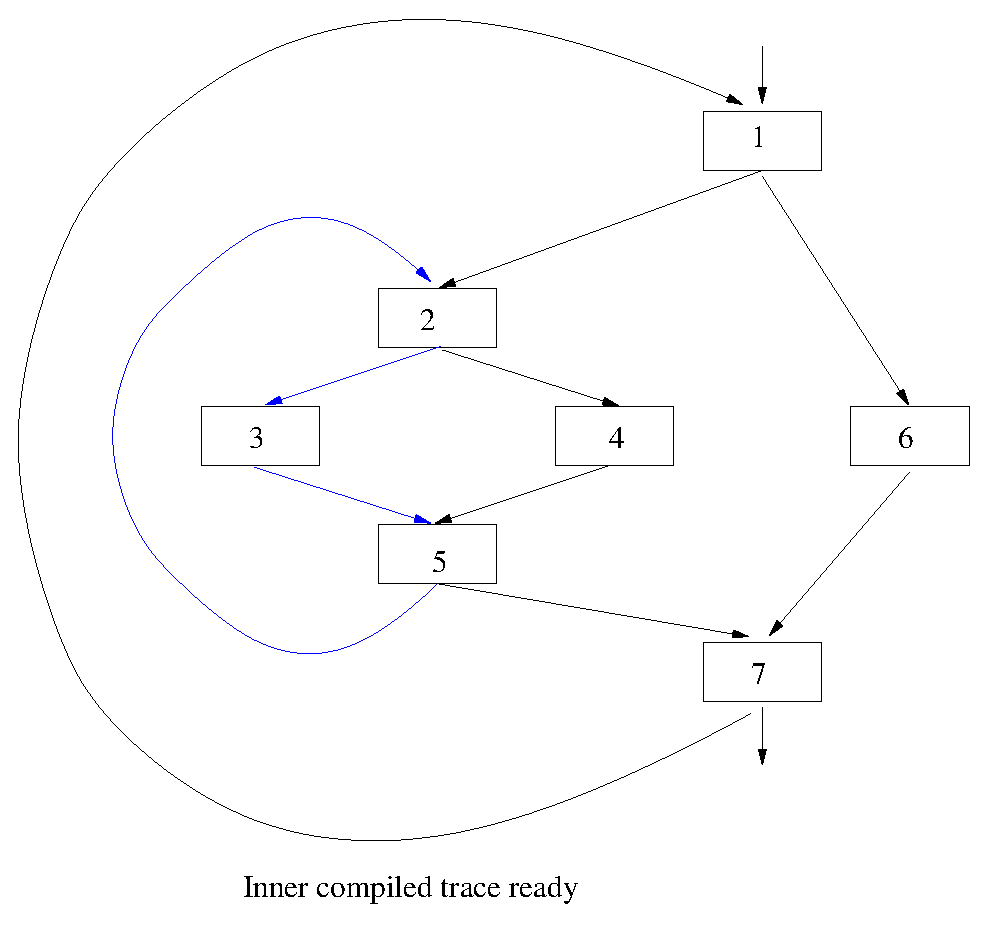
\includegraphics{Figs/3.3.eps}
  }
  \end{figure}
}
\frame
{
  \frametitle{\subsecname}
  \begin{figure}[h]
  \centering
  \scalebox{0.45}{
    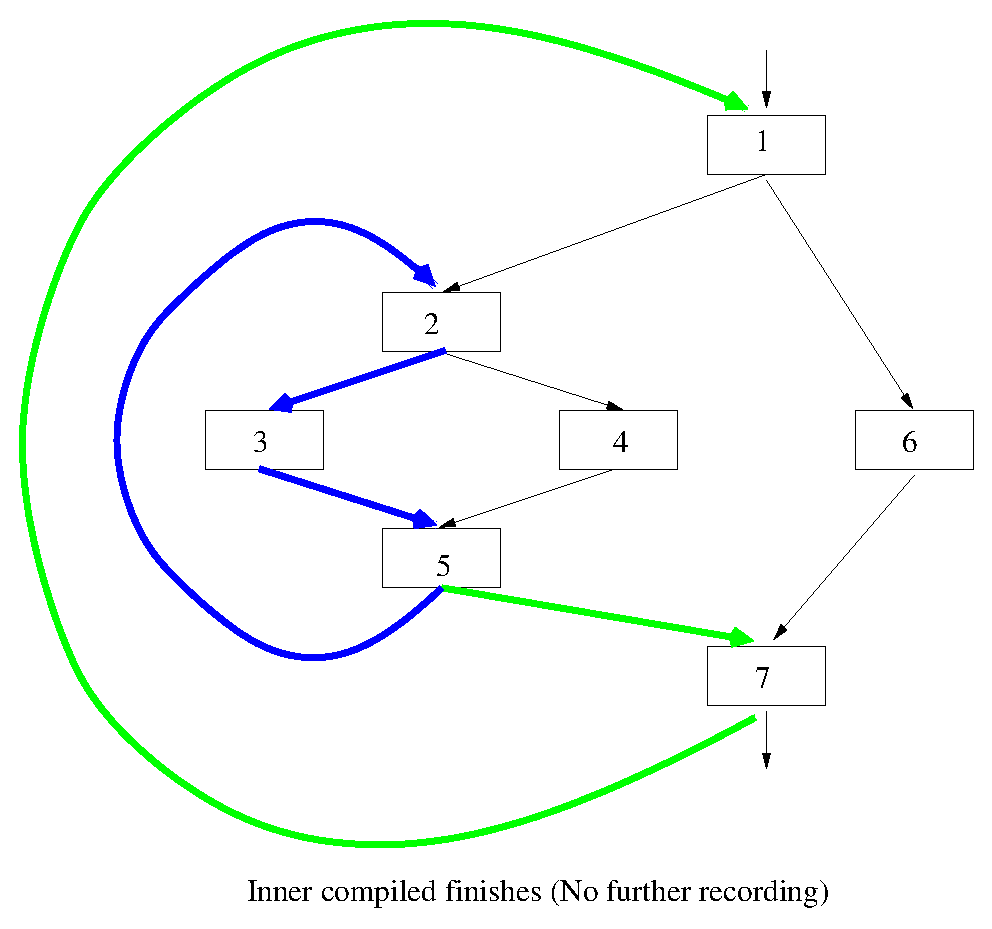
\includegraphics{Figs/3.3.1.eps}
  }
  \end{figure}
}
\frame
{
  \frametitle{\subsecname}
  \begin{figure}[h]
  \centering
  \scalebox{0.45}{
    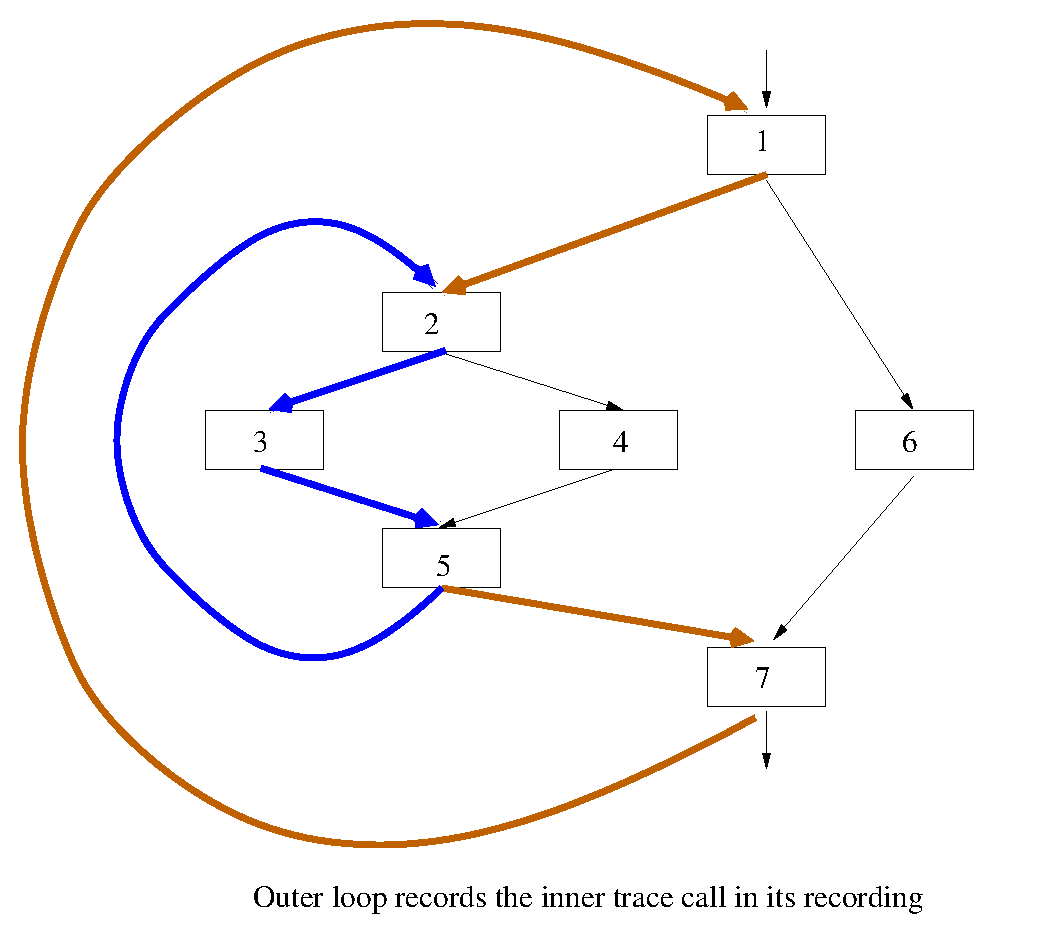
\includegraphics{Figs/3.4.eps}
  }
  \end{figure}
}
\frame
{
  \frametitle{\subsecname}
  \begin{figure}[h]
  \centering
  \scalebox{0.45}{
    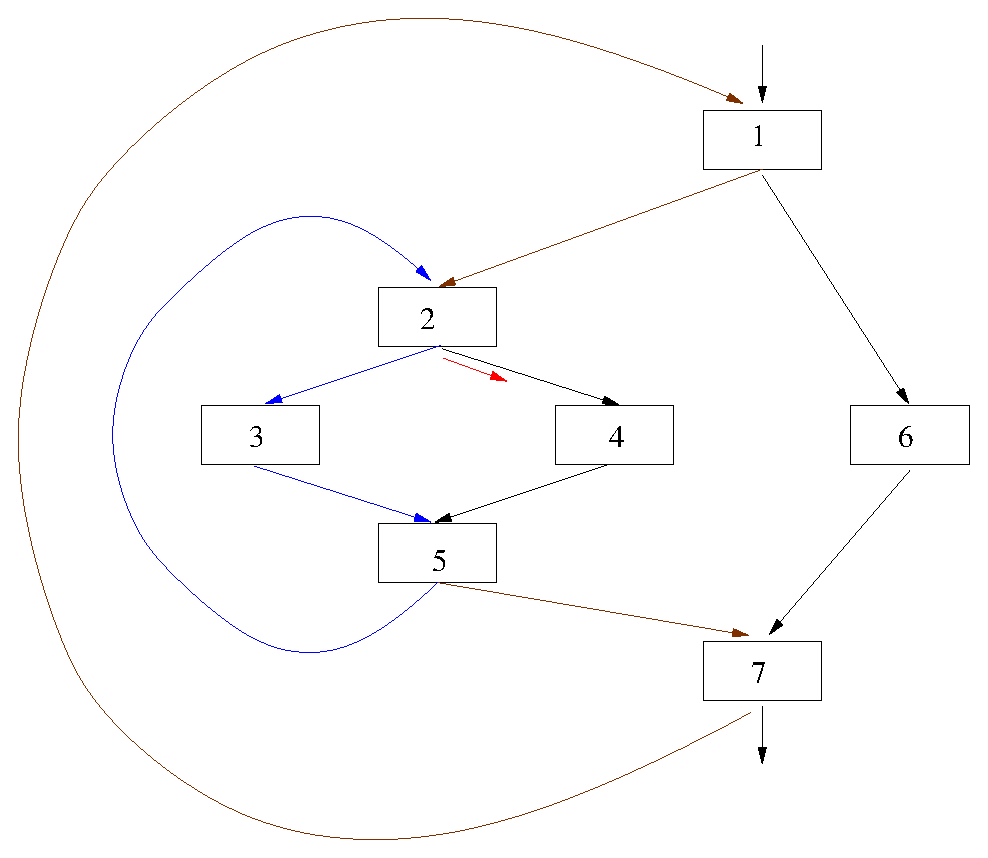
\includegraphics{Figs/3.4.1.eps}
  }
  \end{figure}
  What if during recording of outer loop, the inner trace got a side exit !!
}
\frame
{
  \frametitle{\subsecname}
  \begin{figure}[h]
  \centering
  \scalebox{0.45}{
    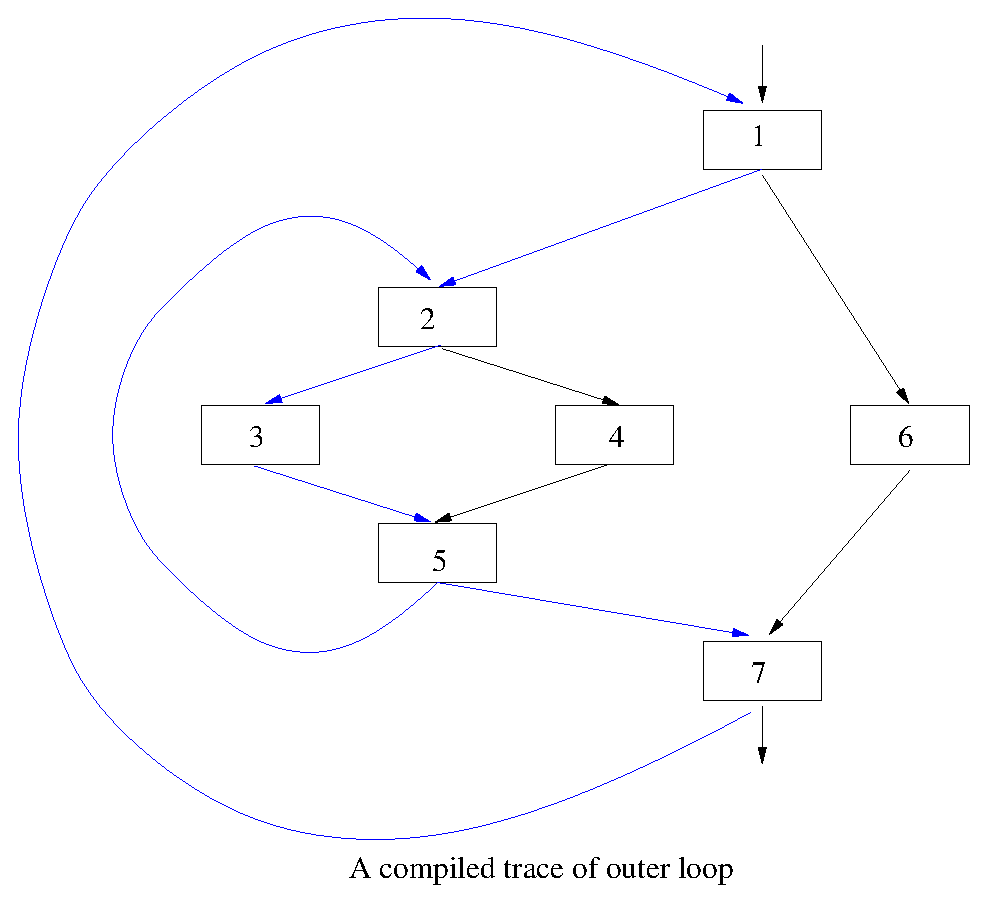
\includegraphics{Figs/3.5.eps}
  }
  \end{figure}
}
\frame
{
  \frametitle{\subsecname}
  \begin{figure}[h]
  \centering
  \scalebox{0.45}{
    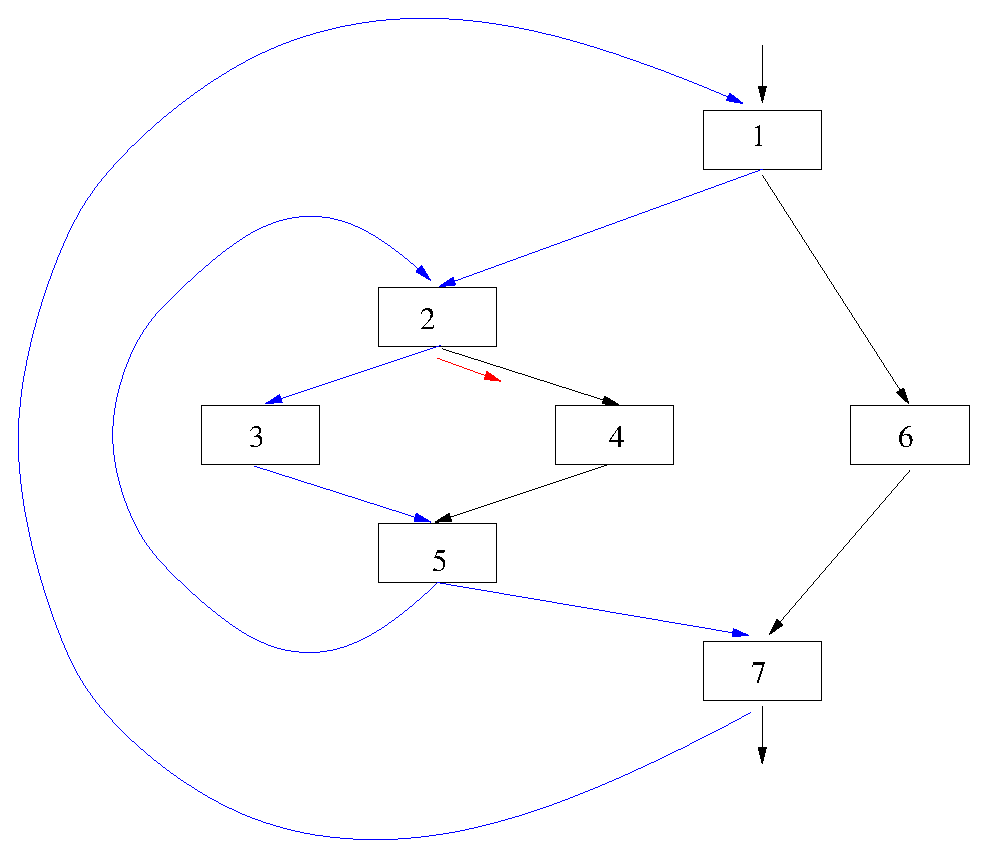
\includegraphics{Figs/3.5.1.eps}
  }
  \end{figure}

  What if during execution of outer loop, the inner trace got a side exit !!
}
\subsection{Modified Blacklisting with Nesting}
\frame
{
  \frametitle{\subsecname}
  \begin{itemize}
   \item  The outer loop blacklisted very quickly.
   \uncover<2> { \item Solution : Blacklist with an option of ``forgiving''  }
   \end{itemize}
}
               \cmt{ as the inner loop not available or takes side exit
   Solution : Increment blacklist counter on such aborts, and backoff on compiling it,  but decrement it when the inner loop
     succesfully finishes a trace and undo the backoff.
               }

\section{Trace Tree Recording \& Optimization}
\subsection{Recording}
\frame
{
  \frametitle{\subsecname}
  \begin{itemize}
    \item While interpreting traces are recorded and transformed into LIR. WHY ?? 
      \begin{itemize}
        \uncover<2> {  \item LIR traces are type specialized}
        \uncover<3> {  \item LIR traces are representation specialized w.r.t objects}
        \uncover<4> { \item LIR traces are representation specialized w.r.t numbers} 
        \uncover<5> { \item LIR traces inline functions}
      \end{itemize}  
    \uncover<6> { \item All the above LIR features need guards}
  \end{itemize}  
}

\subsection{Trace Tree Optimization}
\frame
{
  \frametitle{\subsecname}
  \begin{itemize}
    \item Optimization Goal: Make compilation fast. (Done by NanoJIT)
    \begin{itemize}
      \uncover<2> {  \item Retrict to small set of optimization }
      \uncover<3> {  \item Avoid any reordering optimizations } 
      \uncover<4> {  \item leverage the fact that the LIR is in SSA form } 
    \end{itemize}
    \uncover<5> {  \item Optimizations are performed in 2 phases: forward and backward } 
  \end{itemize}     
}

\subsection{Forward Optimizations}
\frame
{
  \frametitle{\subsecname}
  \begin{itemize}
    \item While recording on each instruction basis.
      \begin{itemize}
        \uncover<2> {  \item Constant subexpression elimination}
        \uncover<3> {  \item Expression simplification and algebraic identities}
        \uncover<4> {  \item ISA specific simplification}
      \end{itemize}  
  \end{itemize}  
}
\subsection{Backward optimizations}
\frame
{
  \frametitle{\subsecname}
  \begin{itemize}
    \item When recording is complete.
    \begin{itemize}
      \uncover<2> {   \item dead data-stack store elimination}
      \uncover<3> {   \item dead call-stack store elimination}
      \uncover<4> {   \item dead code elimination}
      \uncover<5> {   \item Register Allocation } 
    \end{itemize}  
  \end{itemize}    
}

\section{Evaluation}
\subsection{Setup}
\frame
{
  \frametitle{\subsecname}
  \begin{itemize}
    \item SunSpider Benchmark suite is used
    \begin{itemize}
        \item SpiderMonkey: JS interpreter. \textbf{Baseline for comparision}
        \item TraceMonkey: The proposed compilation strategy
        \item SquirrelFish Extreme (SFX): Call threaded JS interpreter
        \item V8: Method compiling JS VM
    \end{itemize}
  \end{itemize}
}
\subsection{Results}
\frame
{
  \frametitle{\subsecname}
  \begin{itemize}
    \item Speed up spreads between 0.9 and 25. 
    \item Speed depends on
    \begin{itemize}
      \item Fraction of bytecode executed as native trace. Not enough!!
      \item Compilation time
    \end{itemize}
  \end{itemize}
}

\subsection{Results Continued}
\frame
{
  \frametitle{\subsecname}
  \begin{itemize}
    \item Overall performance speedup of native trace execution  = $\frac{\text{Time per bytecode execution in Interpreter}}{\text{Time per bytecode execution in native code}  } = 3.9$
      \cmt{
    \item Native trace takes 9 cycles/ byte code as compared to the interpreter ( 35 cycle/ bytecode) 
      }
    \item Other VMs have an overall performance speedup of 3.0
    \item TraceMonkey recording \& compilation 200 times slower than interpreter speed.
  \end{itemize}
}
\subsection{My Critique}
\frame
{
  \frametitle{\subsecname}
  \begin{itemize}
  \cmt{
    \item Web as Desktop
      In short, plenty. JavaScript has become a predominant technology amongst today's web developers, and Mozilla—along with pretty much every web browser maker out there—aims to make it just as fast as code that runs on your desktop. The closer everyone gets to that kind of speed, the closer the idea of the Web as Desktop gets to reality. This is handily demonstrated in a video demonstration of online photo editing over at Mozilla's site. With just-in-time compiling, actions the user takes on a web program move along as if being adjusted in a desktop app, as opposed to having to basically re-load an entire JavaScript app and figure out what state it's in.}
    \item Incremental recompilation.
  \end{itemize}
}

\section{Questions?}
\subsection{Questions?}
\frame
{}

\section{Backup Slides?}
\subsection{Correctness}
\frame
{
  \frametitle{\subsecname}
  \begin{itemize}
    \item Mozilla’s JavaScript fuzz tester, JSFUNFUZZ, random test generator.
    \item Modified JSFUNFUZZ to generate
    \begin{itemize}
      \item loops
      \item type unstable loops
      \item heavy branching code.
    \end{itemize}
  \end{itemize}
}
\subsection{Implementation}
\frame
{
  \frametitle{\subsecname}
  \begin{itemize}
    \item Implemented for SpiderMonkey JS virtual machine.
    \item SpiderMonkey is the interpreter for JS
    \item first compiled into bytecode, then interpreted.
    \item is garbage collected (non-generational, stop the world, mark and sweep)
  \end{itemize}  
}
\subsection{Calling compiled trace}
\frame
{
  \frametitle{\subsecname}
  \begin{itemize}
    \item traces are stored in a trace cache indexed by interpreter PC and type map.
    \item traces are compiled so that they can be called as functions using standard native calling conventions.
  \end{itemize}  
}
\end{document}

\cmt{
1. Before the running exmpl tell what is recording.
  by recording while recording the VM is interreting the code and at the same time convert the bytecode into a low level intermediate 
  representation.
  2. Backward opt rewuire backward program analysis
  2. does the speedup conform to Amdahls law
  3. Type stable loop handling tell about when that can happen

}

\cmt{
\subsection{Register Allocation}
\frame
{
  \frametitle{\subsecname}
  \begin{itemize}
    \item Local register allocator
    \item Any time a value needs to be stored in register, one is assigned free registers list. 
    \item When all registers are in use, the least-often-used register currently in use is spilled. Motivation ??
  \end{itemize}  
}
    \begin{itemize}  
      \item 9 / 26 : TraceMonkey is the fastest
      \item 5 / 26 : The current implementation does not trace recursion.
      \item 5 / 26 : nested loop with small bodies. May be more time in calling nested trace.
      \item 2 / 26 : Does not trace eval and some other C implememnted functions.
      \item 2 / 26 : Trace well, but long compilation.
      \item 1 / 26 : Does not trace through regular expresion replace operations.
      \item 1 / 26 : run time dominated by string processing buitlins.
      \item 1 / 26 : dominated by regular expression matching (implemented in all 3 VM as special regular expression compiler) 
    \end{itemize}  
}
